\documentclass[12pt, a4paper, twoside]{book}

%%%%%%%%%%%Pacchetti Per Compilazione%%%%%%%%%%%
\usepackage[utf8]{inputenc}
\usepackage{graphicx}
\usepackage[a-1b]{pdfx}
\usepackage[justification=centering]{caption}
\usepackage{subcaption}
\usepackage{fancyhdr} % abstract
\usepackage[english,italian]{babel}
\usepackage{listings}
\usepackage{amsthm}
\usepackage{amsmath}
\usepackage{todonotes}
\usepackage{color}
\usepackage{algorithm}
\usepackage{frontespizio}
\usepackage[noend]{algpseudocode}
\usepackage{tabularx}
\usepackage{hhline}
\usepackage[section]{placeins}

\hypersetup{hidelinks}

%%%%%%%%%%%%%%%%%%%%%%%%%%%%%%%%%

%%%%%%%%%%%Comandi per formattazione%%%%%%%%%%%
%Per mantenere i floats (immagini, tabelle etc.) all'interno delle sottosezioni
\makeatletter
\AtBeginDocument{%
	\expandafter\renewcommand\expandafter\subsection\expandafter{%
		\expandafter\@fb@secFB\subsection
	}%
}
\makeatother

%Label in italiano
\makeatletter
\renewcommand{\ALG@name}{Algorithm}
\makeatother

\renewcommand{\lstlistingname}{Listing}

\renewcommand{\listalgorithmname}{List of algorithms}

%Pagina bianca post capitolo effettivamente vuota e senza header
\let\origdoublepage\cleardoublepage
\newcommand{\clearemptydoublepage}{%
	\clearpage
	{\pagestyle{empty}\origdoublepage}%
}
\let\cleardoublepage\clearemptydoublepage

%%%%%%%%%%%%%%%%%%%%%%%%%%%%%%%%%

%%%%%%%%%%%Gestione Codice in Listings (Per C++)
\definecolor{mygreen}{rgb}{0,0.4,0}
\definecolor{mygray}{rgb}{0.35,0.35,0.35}
\definecolor{mymauve}{rgb}{0.58,0,0.82}

\lstset{ %
	backgroundcolor=\color{white},   % choose the background color; you must add \usepackage{color} or \usepackage{xcolor}
	basicstyle=\footnotesize,        % the size of the fonts that are used for the code
	breakatwhitespace=false,         % sets if automatic breaks should only happen at whitespace
	breaklines=true,                 % sets automatic line breaking
	captionpos=b,                    % sets the caption-position to bottom
	commentstyle=\color{mygray},    % comment style
	deletekeywords={...},            % if you want to delete keywords from the given language
	escapeinside={(*@}{@*)},          % if you want to add LaTeX within your code
	extendedchars=true,              % lets you use non-ASCII characters; for 8-bits encodings only, does not work with UTF-8
	frame=no,	                 % adds a frame around the code
	keepspaces=true,                 % keeps spaces in text, useful for keeping indentation of code (possibly needs columns=flexible)
	keywordstyle=\color{mygreen},       % keyword style
	% language=C++,                    % the language of the code
	otherkeywords={*,...},           % if you want to add more keywords to the set
	numbers=left,                    % where to put the line-numbers; possible values are (none, left, right)
	numbersep=5pt,                   % how far the line-numbers are from the code
	numberstyle=\tiny\color{black}, % the style that is used for the line-numbers
	rulecolor=\color{black},         % if not set, the frame-color may be changed on line-breaks within not-black text (e.g. comments (green here))
	showspaces=false,                % show spaces everywhere adding particular underscores; it overrides 'showstringspaces'
	showstringspaces=false,          % underline spaces within strings only
	showtabs=false,                  % show tabs within strings adding particular underscores
	stepnumber=1,                    % the step between two line-numbers. If it's 1, each line will be numbered
	stringstyle=\color{black},     % string literal style
	tabsize=2,	                   % sets default tabsize to 2 spaces
	title=\lstname, % show the filename of files included with \lstinputlisting; also try caption instead of title
	literate={``}{\textquotedblleft}1,
  deletestring=[b]",
}


%%%Macro per pseudocodice
\newcommand*\Let[2]{\State #1 $\gets$ #2}
%%%%%%%%%%%%%%%%%%%%%%


%%%%%%%%%%%Gestione Headers
\newcommand{\fncyblank}{\fancyhf{}}
\pagestyle{fancy}
\fancyhead{}
\fancyhead[LE, RO]{\leftmark}

\begin{document}

\selectlanguage{english}
%%%% Il frontespizio
%Per modificare:
% 1) Modifica Frontespizio/Frontespizio.tex
% 2) Compila Tesi (questo file)
% 3) Compila Tesi-frn.tex
% 4) Ricompila Tesi (questo file)
\begin{frontespizio}
	\Margini {3cm}{3cm}{3cm}{3cm}
	\Istituzione{}
	\Logo[6cm]{Immagini/logo_unipr.png}
	\Dipartimento{Scienze Matematiche, Fisiche e Informatiche}
	\Corso[Laurea Triennale]{Informatica}
	\Annoaccademico{2021-2022}
	\Titoletto{Tesi di Laurea}
	\Titolo {\uppercase {Integrating ECLAIR static analysis in IDEs using the Language Server Protocol}}
	\Sottotitolo{Integrazione dell'analizzatore statico ECLAIR in IDE tramite il Language Server Protocol}
	\Candidato{Nicolò Fuccella}
	\Relatore{Prof. Roberto Bagnara}
\end{frontespizio}




\cleardoublepage

\chapter*{Abstract}
\pagenumbering{gobble}
ECLAIR is a powerful platform for software verification with a strong focus on the development of high-integrity systems, including safety-and security-critical systems. ECLAIR works on the desktop and on the server to analyze entire projects to find possible defects. Following the ``shift-left'' trend (that is, performing verification activities starting from the early development phases), the work described in this thesis aims at providing a proof-of-concept of ``immediate feedback software verification'' using ECLAIR. This entails giving feedback to developers about their code correctness while they're writing the code, directly in the IDE they use for development and without slowing down their work.
One of the challenges to be faced is the compatibility with multiple IDEs and editors. The proliferation of such coding environments, each one with its own extension standards and practices, urges a decoupling between the IDE's extension/plugin interface and the verification-specific smarts. The Language Server Protocol aims precisely at that: having a standardized protocol for communications between a Language Server and the IDE, a single Language Server can be reused for multiple development environments.
The transition from the traditional way in which static analysis results are consumed to this ``immediate feedback'' modality presents another challenge: analysis time becomes critical and a fully satisfactory solution requires sophistication in the static analysis techniques (such as incrementality and parallelism).
We developed a proof-of-concept implementation of the integration of ECLAIR with IDEs using the Language Server Protocol. This thesis describes the underlying ideas, the challenges, the possible solutions explored during the implementation of the proof-of-concept, the lessons learned, and the further developments that, in our opinion, have the potential of turning the prototype into a fully fledged software development tool.


\cleardoublepage

\chapter*{Sommario}
\pagenumbering{gobble}
ECLAIR è un potente strumento per la verifica del software focalizzato sullo sviluppo di sistemi high-integrity, safety-critical e security-critical. ECLAIR è pensato per funzionare sia sul desktop che sul server per analizzare interi progetti al fine di rilevarne eventuali difetti. Seguendo la tendenza verso il cosiddetto ``shift-left'' (che consiste nell'anticipare le attività di verifica già dalle prime fasi dello sviluppo), il progetto descritto in questa tesi ha l'obiettivo di fornire una prova di fattibilità di un ``sistema di verifica con feedback immediato'' usando ECLAIR. Questo al fine di dare feedback agli sviluppatori in merito alla correttezza del loro codice durante la stesura del programma, direttamente dall'IDE che già utilizzano per lo sviluppo e senza subire rallentamenti.
Una delle sfide da affrontare in un progetto di questo tipo è garantire la compatibilità con i vari IDE ed editor. La proliferazione di questi ambienti di sviluppo, ciascuno con i suoi standard e approcci consigliati per la realizzazione di estensioni, rende necessaria una separazione tra l'interfaccia dell'estensione/plugin dell'IDE e le funzionalità prettamente legate all'analisi. Il Language Server Protocol si pone come obiettivo precisamente questo: definendo un protocollo standardizzato per le comunicazioni tra un Language Server e l'ambiente di sviluppo, un solo Language Server può essere utilizzato per vari ambienti di sviluppo senza apportare modifiche.
Il passaggio dal tradizionale approccio alla fruizione dei risultati dell'analisi statica a questa modalità ``con feedback immediato'' presenta altre sfide: il tempo di analisi diventa un fattore determinante e la realizzazione di una soluzione richiede l'impiego di alcune tecniche di analisi piuttosto sofisticate (per esempio incrementalità e parallelismo).
Abbiamo realizzato un'implementazione che costituisce una prova di fattibilità dell'integrazione di ECLAIR in alcuni ambienti di sviluppo usando il Language Server Protocol. Questa tesi ha l'obiettivo di descrivere le idee sottostanti, le sfide affrontate, le possibili soluzioni esplorate durante l'implementazione del prototipo, gli insegnamenti appresi, e i futuri sviluppi che, a nostro avviso, hanno il potenziale di trasformare il prototipo in uno strumento di sviluppo software a pieno titolo.


\cleardoublepage

%%%% Gli indici
\pagestyle{plain}
\pagenumbering{roman}
\tableofcontents
%

\listoffigures    %Commentare se non vi sono Immagini
%
%
%
%%%% La prefazione
\chapter*{Introduction} %Se si cambia il Titolo cambiare anche la riga successiva così che appia corretto nell'indice
\addcontentsline{toc}{chapter}{Introduction} %Per far apparire Introduzione nell'indice (Il nome deve rispecchiare quello del chapter)
\pagenumbering{arabic} % Settaggio numerazione normale
Nowadays static analysis is more and more common in every development scenario. In some cases, especially safety-critical ones, it is even enforced by regulation and industry standards. Although it can improve code quality dramatically, developers are often reluctant to implement it. This is mainly due to the fact that most of these tools are designed to run separately from development environments: they return extensive lists of notifications which must be inspected one by one in a time-consuming fashion. 
Analyzers manufacturers know the situation and tried different approaches: it is now common for them to build on top of their existing tools integrations with IDEs and CI (Continuous Integration) pipelines.
The core of the analyzer and its code remains pretty much the same, what changes is the interface that the end users can rely on.
This thesis focused on the integration possibilities between the IDE and the analyzer, in order to assist the user during the coding.
This can be achieved in different ways: from a simple button in the IDE that triggers the analysis to more integrated experiences.
\\\\
In a publication by Yuriy Tymchuk, Mohammad Ghafari and Oscar Nierstrasz in occasion of the 2018 IEEE/ACM 26th International Conference we can read:
\begin{quote}
\itshape
``We learned that the availability of our tool as a default IDE feature and its automatic execution are the main reasons for its adoption. Moreover, the fact that immediate feedback is provided directly in the related development context is essential to keeping developers satisfied, although in certain cases feedback delivered later was deemed more useful.'' \cite{8973102}
\end{quote}

This confirmed our hunch, and we wanted to try to build an IDE extension on top of an existing analyzer, ECLAIR by BUGSENG\footnote{https://www.bugseng.com/eclair}, to better understand the challenges and the state of the art of this kind of integration.
BUGSENG had already explored integrations with CI pipelines and the analyzer was already capable of exporting reports in different formats: given this background we could fully concentrate on the IDE side.
After a brief analysis of other tools and developer feedback, we outlined the experience we wanted to present to the users: they should still be able to trigger an analysis manually, but in addition to that whenever a file was changed or opened for the first time, it should run automatically, so that we could always present the most updated warnings to the user.
However, each IDE has its own primitives and APIs to be called in order to integrate the functionalities we wanted. 
It would have been time consuming and a maintenance nightmare to develop extensions for all the mostly used IDEs, until we learned about the Language Server Protocol\footnote{https://microsoft.github.io/language-server-protocol}: defining a common communication standard between the IDE and a decoupled Language Server, the protocol handles the heavy lifting of reducing all the IDEs to a common interface from the server point of view.
This way we could integrate the analysis smarts in the Language Server, who could seamlessly deliver the warnings to the IDE, and fully concentrate on problems like incrementality and parallelism.
\\\\
After some initial experiments, we built a prototype of a VSCode extension which relies on the Language Server Protocol for all the communication between a Language Server and the IDE. The Language Server behaves as an orchestrator between two tools: the ECLAIR analyzer itself and \emph{eclair\textunderscore	report}, which serves the violations met.
\\\\
We believe that tools like this, which entails performing the analysis during the software development phase, can give an important boost to developers and allow them to conciliate speed and code quality assuring that bugs, inconsistencies, design issues and other quirks won't reach the production environment, but will be dealt with before.

%

\pagestyle{fancy}

\part{Preliminary Notions}\label{part:preliminary-notions}
This part of the thesis introduces the main preliminary notions and premises that are needed for the presentation of the contents of Part 2, and that provide the reader with the necessary context information.
\\\\
In Chapter~\ref{chapter:verifying-the-correctness-of-programs}, the current approaches at verifying the correctness of programs are presented. After an introduction about testing in general, the reasons behind static analysis are presented and the pros and cons are weighed. 
\\\\
Chapter~\ref{chapter:shift-left-testing} will then focus on shift-left testing movement and what it actually implies.
\\\\
Moving to Chapter~\ref{chapter:eclair}, the ECLAIR static analyzer is presented, on top of which the proof-of-concept has been realized. Before talking about integrating ECLAIR static analysis in IDEs, it is important to understand how ECLAIR works and the reasoning behind it. Chapter~\ref{chapter:eclair} also includes an introduction to MISRA C and its guidelines.
\\\\
Lastly, Chapter~\ref{chapter:language-server-protocol} presents the Language Server Protocol on top of which all the communications between the IDEs and the analysis system are performed. Thanks to this protocol, we were able to decouple the IDEs extensions from the analysis tools.
\chapter{Verifying the Correctness of Programs}\label{chapter:verifying-the-correctness-of-programs}
Today's dominant practice in the software industry is to demonstrate the correctness of programs empirically. Some inputs are fed to the tested program and the correctness of the output is verified against expected ones. In some cases exhaustive testing is possible, but in large software it generally is not. Just focusing on a single function, for example, with one 32-bit parameter it can possibly be exhaustively tested.  With more than one 32-bit parameters or one or more 64-bit parameters, exhaustive testing suddenly becomes impossible.

However, the only thing we can actually prove with such an approach is that the program is incorrect: a single instance of incorrect behavior suffices to spot a problem. Unfortunately, when there is not an observation of incorrect behavior, we cannot know whether the program is correct or we have just not tested it with an input that would trigger an error.
Some more sophisticated testing tries to choose the inputs so that all, or at least the majority of the possible execution paths are examined, and to test modules or units (testing in the small) as well as the overall software behavior (testing in the large). 
\\\\
Regardless of how sophisticated the testing is, empirical methods do not actually prove that a program is correct.
Adopting a completely different approach, static analysis aims at giving more insights about some properties of the program without the need for the execution, but by examining the code.
An analyzer scans all the code in a project, understands its structure and helps to check for vulnerabilities and ensure that it adheres to industry standards. 
So static analysis is mostly useful when looking for:
\begin{itemize}
  \item security vulnerabilities;
  \item programming errors;
  \item coding standard or syntax violations;
  \item performance issues.
\end{itemize}

Integrating static analysis in the development workflow improves code quality, thanks to automated tools which are less prone to human error, increase the likelihood of finding vulnerabilities and, paired with normal testing methods, allows for more depth into debugging code.

However, static analysis comes with some drawbacks such as false positives and sometimes cryptic violation reports. In addition, enforcing too strict coding rules may slow down the development for little benefit.
\\\\
Nowadays static analysis is a mandatory step in high level software development, in particular for safety-critical systems and is often enforced by common regulations. Thus we have seen a proliferation of such tools, which are commonly paired with code review automations and continuous integration pipelines on platforms like GitHub\footnote{https://github.com} or Gitlab\footnote{https://gitlab.com}. These integrations perform the analysis after the code has been written or at least when it has reached a stable state (usually when changes are pushed to the repository or a pull request is opened). 
Some of these tools are used also during the code writing to improve the quality and reduce the errors before shipping the changes and performing more in-depth checks. 
This last use case opens a series of new requirements and problems: first of all, performing the analysis in the shortest amount of time becomes of the utmost importance, and while it is doable for short files, sometimes the codebases to consider can be huge and with a number of levels of abstractions. The analysis tooling, in order to be effective, must become a shared habit across the team, thus giving space to additional headaches: teams work on different platforms (Linux, MacOS, Windows, etc…) and with different IDEs/editors (Intellij Idea\footnote{https://www.jetbrains.com/idea}, VSCode\footnote{https://code.visualstudio.com} and Emacs\footnote{https://www.gnu.org/software/emacs} just to name a few). Acknowledging that, the static analysis tools must be compatible with each of them, with an increase in the number of softwares to be developed and maintained by the producers. 

\chapter{Shift-left testing}\label{chapter:shift-left-testing}
In an article dated September 1st 2001 appeared in Dr. Dobb's Journal, Larry Smith wrote: 
\begin{quote}
\itshape
``Shift-left testing is how I refer to a better way of integrating the quality assurance (QA) and development parts of a software project.  By linking these two functions at lower levels of management, you can expand your testing program while reducing manpower and equipment needs - sometimes by as much as an order of magnitude.'' \cite{10.5555/500399.500404}
\end{quote}
This article is considered the manifesto of the shift-left movement, which is about moving the testing phase earlier in the software development lifecycle, shifting-left.

To give some background to the reader, up until the late 1990s, a typical software development process was sequential: the design was followed by the development, while testing and deployment were the latest phases of the project lifetime. Placing the testing phase at a late stage, bug fixing was costly and time-consuming. Sometimes developers had to even fully redesign the application in order to make everything behave correctly.
Kent Beck and Cynthia Andres wrote about this 
\begin{quote}
\itshape
``Here is the dilemma in software development: defects are expensive, but eliminating defects is also expensive. However, most defects end up costing more than it would have cost to prevent them.'' \cite{beck2004extreme}
\end{quote}

\begin{figure}[ht]
	\centering
	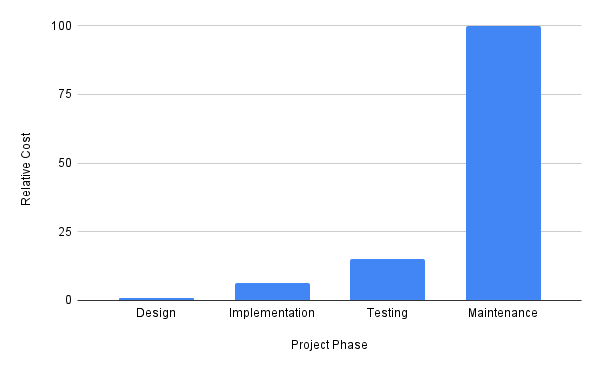
\includegraphics[width=1.0\textwidth]{Immagini/relative_cost_of_fixing_defects.jpg}
	\caption{Relative Cost of Fixing Defects}
	\label{fig:one}
\end{figure}

Listening to Larry Smith's suggestion, more and more teams try to integrate the quality assurance from the earlier phases of the development. The test-driven development is an approach that tries to do exactly this, designing the tests even before beginning the coding part. 
In addition, many tools were born to help the developers to ``shift-left'', like static analyzers. 
\\\\
It is important for the reader to understand that this kind of approach, aside from helping to find bugs early, thus reducing the costs implied by patches and code fixes, leads to a higher-quality product and codebase. This usually can help reduce the time to ship a product, avoiding unexpected issues and the need for refactoring existing parts of the code.
\\\\
In a software industry that is everyday more and more bound to other fields, especially safety-critical ones like medical, automobilistic and aeroespacial just to name a few, software quality is of the utmost importance, hence the \emph{``test early and often''} motto has become kind of a mantra for teams, which has now the instruments to catch defects as early as possible and in the least expensive way by integrating sane good practices and habits during the development.
\chapter{ECLAIR}\label{chapter:eclair}
ECLAIR is a powerful platform for software verification. At the moment of this writing the latest stable release, and the version adopted for the project described in Part~\ref{part:the-proof-of-concept}, is the 3.12.0.
Applications range from coding rule validation, with a particular emphasis on the MISRA and BARR-C coding standards, to the computation of software metrics, to the checking of independence and freedom from interference among software components, to the automatic detection of important classes of software errors.
ECLAIR is certified for use in safety-critical development ranging from automotive to aerospace use cases, moving to industrial and medical ones.
It uses formal methods-based static code analysis techniques such as abstract interpretation and model checking combined with constraint satisfaction techniques to detect or prove the absence of certain run time errors in source code, and provides support for program analysis and verification, program test generation and program transformation.

\begin{figure}[ht]
	\centering
	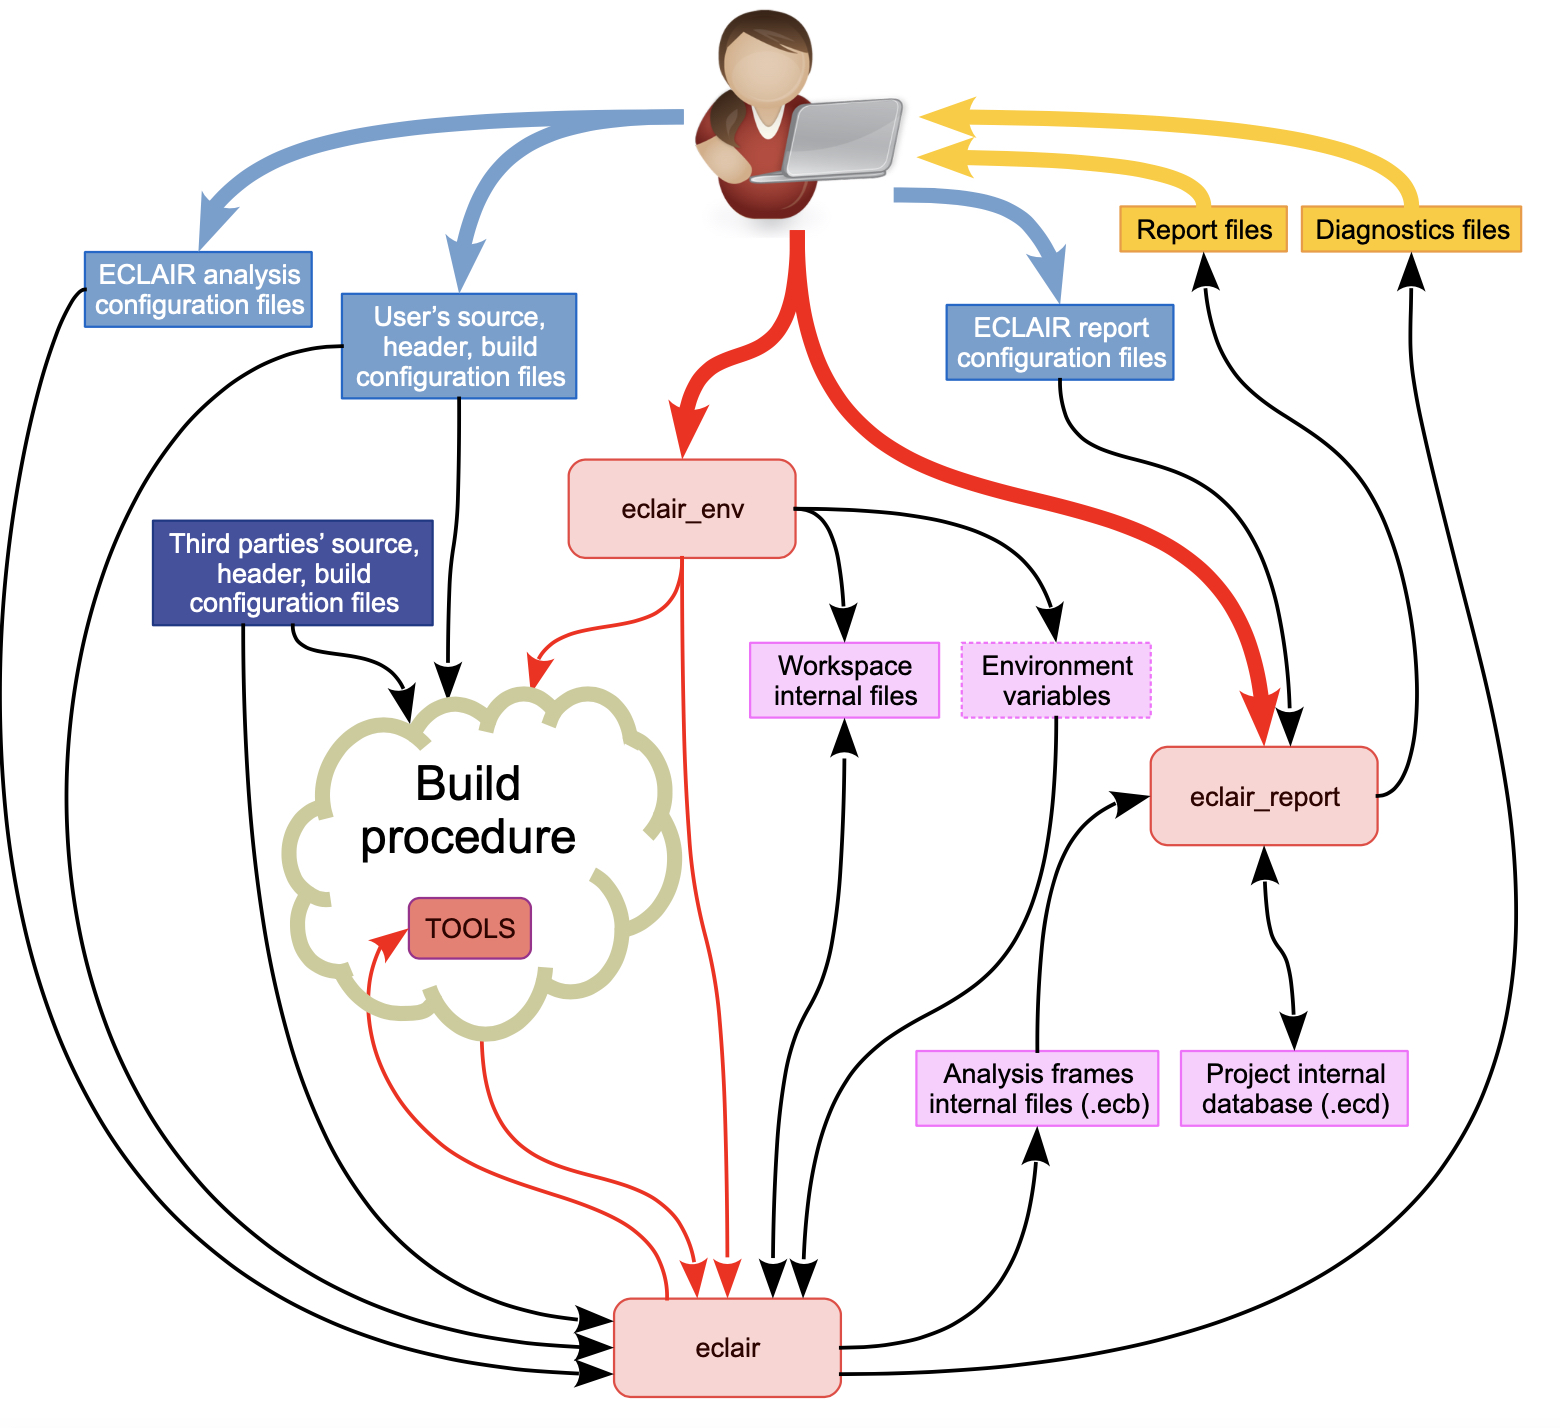
\includegraphics[width=1.0\textwidth]{Immagini/ECLAIR_basic_qualifiable_architecture.jpg}
	\caption{ECLAIR basic qualifiable architecture - Image copyright by BUGSENG srl, reproduced with permission.}
	\label{fig:one}
\end{figure}

\section{Abstract interpretation}
Abstract interpretation was formalized by the French computer scientists Patrick Cousot and Radhia Cousot in the late 1970s and it mainly consists of the automatic extraction of information about the possible execution paths of a program.
The formalization of all these possible execution paths is called \emph{concrete semantics}. The concrete semantics of a program is, in general, a non-computable, typically infinite mathematical object. Thus it is not possible to write a program to compute it. Having said that, all the non-trivial questions about the concrete semantics are undecidable. 

However, we can consider a sound approximation of the concrete program semantics, called \emph{abstract semantics}, and reason on it. Since the abstract semantics covers all possible cases, we can use it to demonstrate safety properties of the program.
\\\\
The abstract semantics is an artificial construct aimed at giving a computable approximation of the concrete semantics. It is important to pay attention to the ``direction'' of the approximation: it must ``err on the safe side'' in order to avoid false negatives, though at the expense of allowing false positives. 
However, once a good approximation is available, abstract interpretation can give precious insights into the program properties and inner workings. 

\begin{figure}[ht]
	\centering
	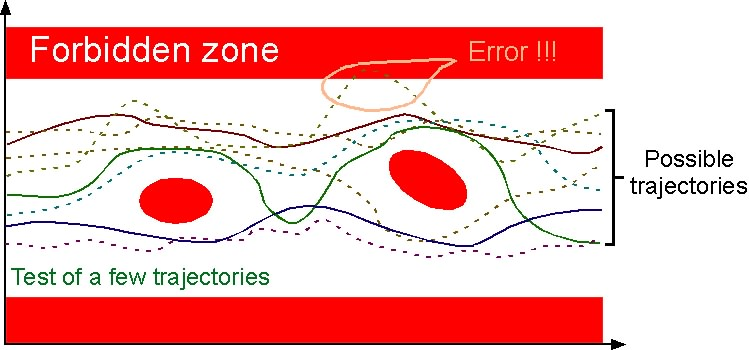
\includegraphics[width=1.0\textwidth]{Immagini/AbstractInterpretationNutshell_trajectories.jpeg}
  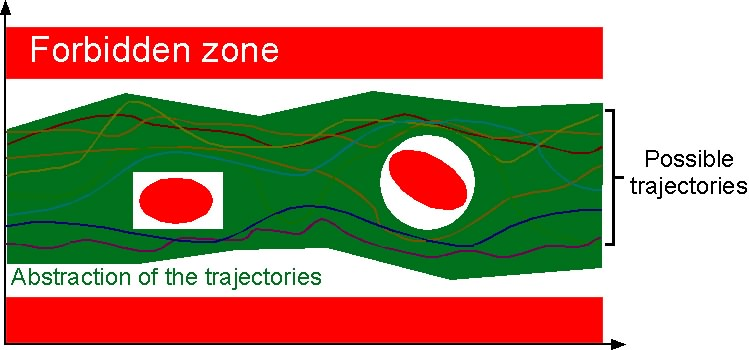
\includegraphics[width=1.0\textwidth]{Immagini/AbstractInterpretationNutshell_interpretation.jpeg}
	\caption{Abstract Interpretation in a Nutshell \cite{AbstractInterpretationNutshell}}
	\label{fig:one}
\end{figure}

\section{Model checking}
Model checking is a method for checking whether a finite-state model of a system meets a given specification (also known as correctness). This verification can be performed by automatically searching the finite state space of the system looking to determine whether the property of the specification is met. To demonstrate that the specification is not met, the checker looks for counterexamples that can give precious insights about the reason for the failure. Having said that, the process of model checking can be summarized as follow:
\begin{itemize}
  \item modeling, which consists of creating an abstract model of the system ignoring all the irrelevant details (eg. through Kripke structures);
  \item specification, which describes with a logical formalism (like temporal logic) properties that must be satisfied;
  \item verification, which checks that the properties are actually met by the system.
\end{itemize}
\begin{figure}[ht]
	\centering
	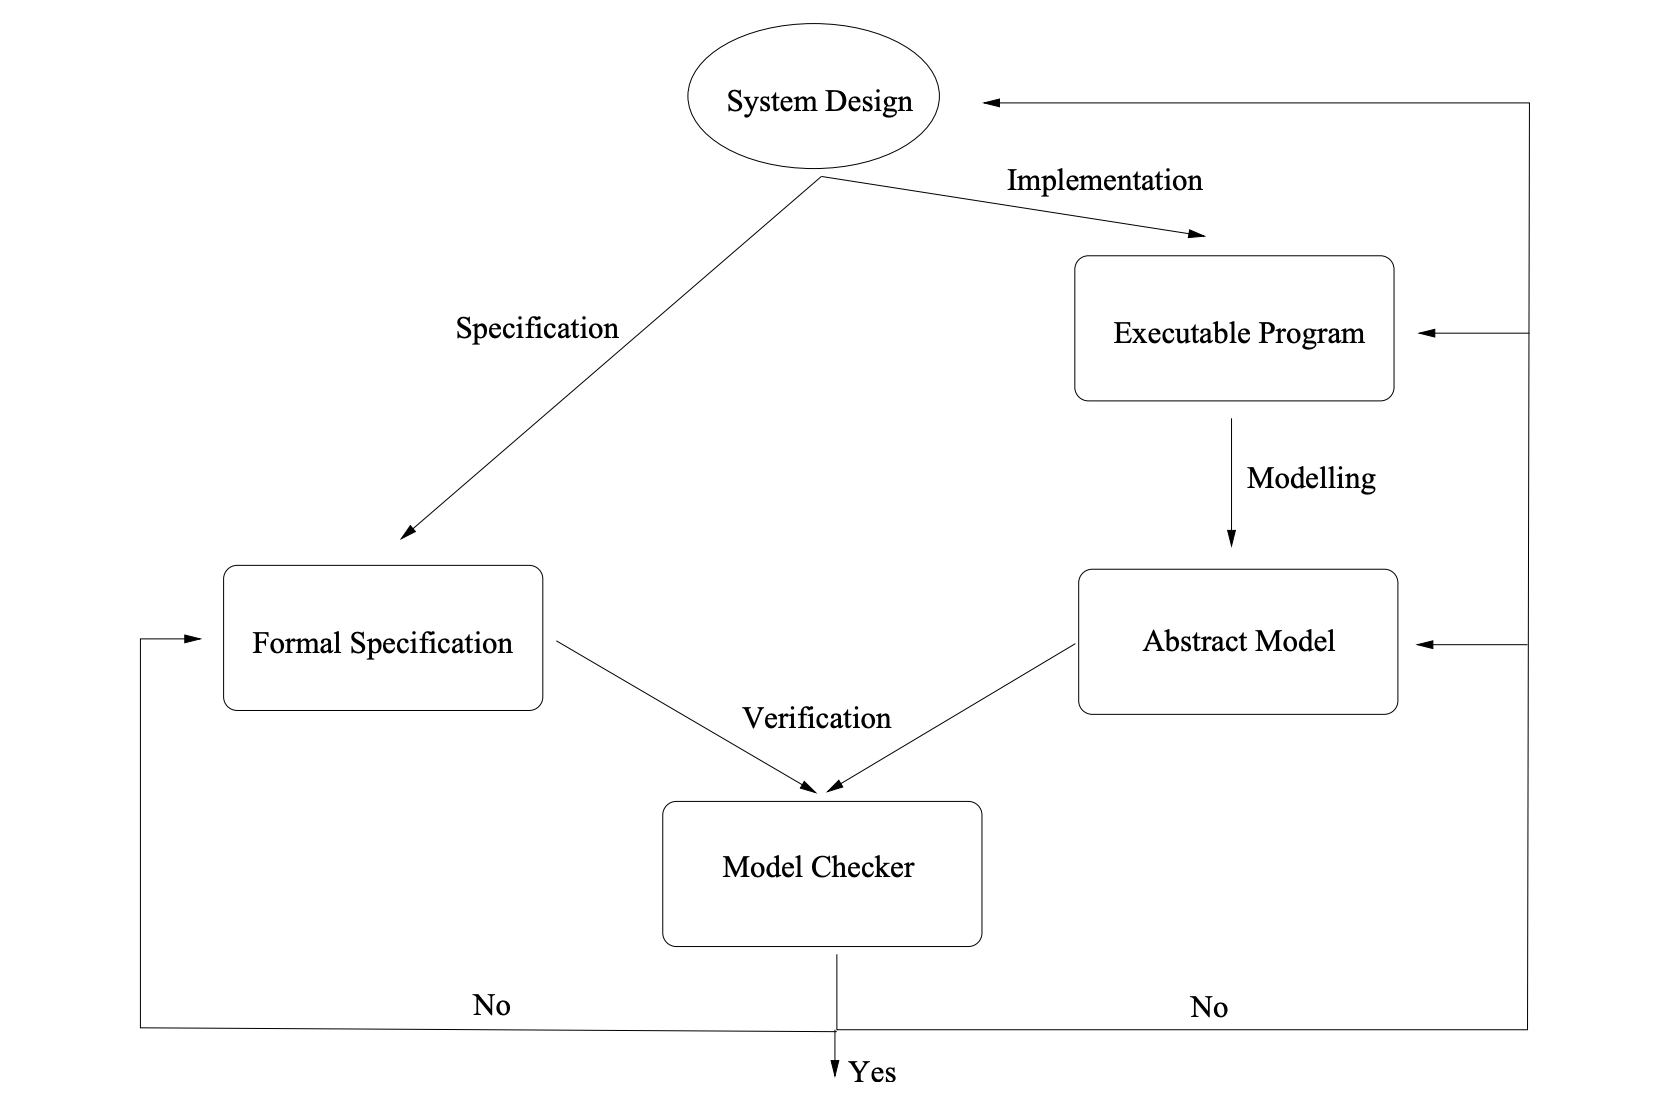
\includegraphics[width=1.0\textwidth]{Immagini/the_process_of_model_checking.jpg}
	\caption{The process of model checking \cite{ModelCheckingProcess}}
	\label{fig:one}
\end{figure}
It is important to pay particular attention to the modeling and specification phases, since errors can make this method give false positives.
Having said that, model checking is a precious method used in several static analysis tools. 

\section{Constraint satisfaction}
Constraint satisfaction is the process of finding a solution through a set of constraints that impose conditions some variables must satisfy.
It is one of the subjects of investigation in the fields of artificial intelligence and operations research.

In particular, Constraint Satisfaction Problems (CSPs) form a specific class of search problems. A CSP is a triple which comprehend:
\begin{itemize}
  \item variables, a finite and non empty set;
  \item domains, finite and non empty sets, one for each variable;
  \item constraints over variables, such that each constraint is a subset of the cartesian product of domains sets.
\end{itemize}
Solutions are combinations of values that can be assigned to the variables, from the respective domains, that satisfies all the constraints at the same time.
\\\\
Constraint satisfaction has also been used to perform checks on programs during static analysis.
Constraint propagation is an essential part of this method, which, relying on local consistency conditions, tries to reduce domains of variables, strengthen constraints, or create new ones. 
To give an idea about the possible use cases of such an approach let's consider an example found in ``A Practical Approach to Verification of Floating-Point C/C++ Programs'' by Bagnara et al. \cite{10.1145/3410875}. 
In Chapter 3 the expression
\begin{quote}
\itshape
float phi\textunderscore = asin(sin(dl) / cosh(ll));
\end{quote}
is translated into static single assignment form and is decomposed. We can read about this:
\begin{quote}
\itshape
``In this intermediate code representation, complex expressions are decomposed into sequences of assignment instructions where at most one operator is applied, and new variable names are introduced so that each variable is assigned to only once.''
\end{quote}
The expression results in a list of statements like this:
\begin{lstlisting}
float phi_; double z1, z2, z3, z4, z5, z6;
z1 = (double) dl;
z2 = sin(z1);
z3 = (double) ll;
z4 = cosh(z3);
z5 = z2/z4;
z6 = asin(z5);
phi_ = (float) z6;	
\end{lstlisting}
and then, regarding line 6:
\begin{quote}
\itshape
``Let us see how this can be used for program verification. As a first example, let us consider the question of whether the division z5 = z2 / z4 can give rise to a division by zero. Assume that all of the intervals are initially full - for instance, they contain all possible numerical floating-point values and all propagators are ready to run. We modify the interval associated to z4 to [-0, +0] and start propagation. At some stage, the indirect propagator for cosh will be called to possibly refine the interval for z3 starting from the interval of z4: a propagator correctly capturing a passable implementation of cosh will refine the label of z3 to the empty interval, thus proving that division by zero is indeed not possible.''
\end{quote}

\section{MISRA C}
MISRA C is a set of software development guidelines and the de facto standard for developing software in C where safety, security and code quality are important. 
It was originally developed to fulfill the need for a ``restricted subset of a standardized programming language'' identified in the 1994 ``Development guidelines for vehicle based software'' and against the background of the emerging use of C for developing embedded software in automotive applications.
Although originally specifically targeted at the automotive industry, it has evolved as a widely accepted model for best practices by leading developers in sectors including automotive, aerospace, telecom, medical devices, defense, railway, and others.
MISRA standards are used to ensure that the code is:
\begin{itemize}
  \item safe;
  \item secure;
  \item reliable;
  \item portable.
\end{itemize}
As we can read in ``A Rationale-Based Classification of MISRA C Guidelines'', Bagnara et al \cite{BagnaraBH22}:
\begin{quote}
\itshape
``Each of the 175 guidelines of MISRA C is classified as being either a \textbf{directive} or a \textbf{rule}:
\\
\textbf{Rule}: a guideline such that information concerning compliance is fully contained in the source code and in the language implementation.
\\
\textbf{Directive}: a guideline such that information concerning com- pliance is not fully contained in the source code and language implementation: requirements, specifications, designs and other considerations may need to be taken into account.

One of the things that is often misunderstood is that MISRA C is much more than just the set of its guidelines. The guidelines are meant to be used in the framework of a documented software development process.
\\\\
...
\\\\
The \textbf{deviation process} is an essential part of the adoption of the MISRA Guidelines, each one of which is assigned a single category: \textbf{mandatory}, \textbf{required} or \textbf{advisory}, defined as follows.

\textbf{Mandatory}: C code that complies with MISRA C must comply with every mandatory guideline: deviation is not permitted.

\textbf{Required}: C code that complies with MISRA C shall comply with every required guideline: a formal deviation is required where this is not the case.

\textbf{Advisory}: these are recommendations that should be followed as far as it is reasonably practical: formal deviation is not required, but non-compliances should be documented.

Whenever complying with a guideline goes against code quality or does not allow access to the hardware or does not allow integrating or use suitably qualified adopted code, the guideline has to be deviated. That is, instead of modifying the code to bring it into compliance, for required guidelines, a written argument has to be provided to justify the violation whereas, for advisory guidelines, this is not necessary.''
\end{quote}
MISRA comprehends a number of rules that are focused mainly on these aspects:
\begin{itemize}
  \item avoiding possible compiler differences;
  \item avoiding using functions and constructs that are prone to failure;
  \item produce maintainable and debuggable code;
  \item best practices in general;
  \item complexity limits.
\end{itemize}
At the moment of this writing there have been three releases of the MISRA C standard:
\begin{itemize}
  \item MISRA C:1998;
  \item MISRA C:2004;
  \item MISRA C:2012.
\end{itemize}
A small selection from the MISRA C 2012 guidelines follows, in order to convey the overall idea of the coding standard:

\noindent\rule{\textwidth}{0.1pt}

\emph{Rule 15.6}:\\

\noindent\fbox{%
    \parbox{\textwidth}{%
      The body of an iteration-statement or a selection-statement shall be a compound-statement
    }%
}
\\\\
\textbf{Category}: Required\\
\textbf{Analysis}: Decidable, Single Translation Unit\\
\textbf{Applies to}: C90, C99\\

It is possible for a developer to mistakenly believe that a sequence of statements forms the body of an iteration-statement or selection-statement by virtue of their indentation. The accidental inclusion of a semi-colon after the controlling expression is a particular danger, leading to a null control statement. Using a compound-statement clearly defines which statements actually form the body.
Additionally, it is possible that indentation may lead a developer to associate an else statement with the wrong if.
\\\\
A famous case in which such a rule would have prevented problems is the ``Apple goto fail vulnerability'': 
on 2014-02-21 Apple released a security update for its implementation of SSL/TLS in many versions of its operating system 
and the indicted code is reported in Listing~\ref{lst:the-apple-goto-fail-vuln}.
\begin{quote}
\itshape
``The problem was the second (duplicate) ``goto fail''. 
The indentation here is misleading; since there are no curly braces after the ``if'' statement, the second ``goto fail'' is always executed. In context, that meant that vital signature checking code was skipped, so both bad and good signatures would be accepted. The extraneous ``goto'' caused the function to return 0 (``no error'') when the rest of the checking was skipped; as a result, invalid certificates were quietly accepted as valid.'' \cite{TheAppleGotoFailVulnerability}
\end{quote}

\begin{lstlisting}[caption={The Apple goto fail vulnerability}, label={lst:the-apple-goto-fail-vuln}]
if ((err = SSLHashSHA1.update(&hashCtx, &signedParams)) != 0)
  goto fail;
  goto fail;
... other checks ...
fail:
  ... buffer frees (cleanups) ...
  return err;
\end{lstlisting}

\noindent\rule{\textwidth}{0.1pt}

\emph{Rule 3.2}:\\

\noindent\fbox{%
    \parbox{\textwidth}{%
    Line-splicing shall not be used in // comments
    }%
}
\\\\
\textbf{Category}: Required\\
\textbf{Analysis}: Decidable, Single Translation Unit\\
\textbf{Applies to}: C99\\

If a // commented line ends with a back-slash followed by a new-line, then the following line is part of the comment, and, if this was not intended, an important line of code maybe lost. 
The following example shows how a seemingly-innocuous path separator at the end of the comment may accidentally comment out the next line of code. \cite{BagnaraBH18}

\begin{lstlisting}[caption={Examples of MISRA C 2012 Rule 3.2 violation and compliance}]
// see critical.* in c:\project\src\
critical_function(); /* Non-compliant */

// see critical.* in c:\project\src
critical_function(); /* Compliant */
\end{lstlisting}

\clearpage

\emph{Rule 9.1}:\\

\noindent\fbox{%
    \parbox{\textwidth}{%
    The value of an object with automatic storage duration shall not be read before it has been set
    }%
}
\\\\
\textbf{Category}: Mandatory\\
\textbf{Analysis}: Undecidable, System\\
\textbf{Applies to}: C90, C99\\

Note that array elements and structure members are considered as discrete objects and they must be (recursively) initialized. 
The rationale is that, according to the C Standard, objects with automatic storage duration are not automatically initialized and can therefore have indeterminate values. Reading them while their value is indeterminate is undefined behavior. \cite{BagnaraBH18}

\noindent\rule{\textwidth}{0.1pt}

\emph{Dir 4.4}:\\

\noindent\fbox{%
    \parbox{\textwidth}{%
      Sections of code should not be ``commented out''
    }%
}
\\\\
\textbf{Category}: Advisory\\
\textbf{Applies to}: C90, C99\\

This rule applies to both // and /* ... */ styles of comment.
Where it is required for sections of source code not to be compiled then this should be achieved by use of conditional compilation (e.g. \#if or \#ifdef constructs with a comment). Using start and end comment markers for this purpose is dangerous because C does not support nested comments, and any comments already existing in the section of code would change the effect.
\chapter{Language Server Protocol}\label{chapter:language-server-protocol}
Implementing support for features like autocomplete, refactoring, navigating to a symbol's definition, syntax highlighting, error and warning markers, or documentation on hover for a programming language is a significant effort. Traditionally this work must be repeated for each development tool, as each provides different APIs for implementing the same features.
The idea behind a Language Server is to provide the language-specific smarts inside a server that can communicate with the development tooling over a protocol that enables inter-process communication.
The Language Server Protocol was originally developed for Microsoft Visual Studio Code and is now an open standard. On 2016 June 27, Microsoft announced a collaboration with Red Hat and Codenvy to standardize the protocol's specification and it is now hosted and developed on GitHub.
The idea behind the Language Server Protocol (also called LSP from now on) is to standardize the protocol used by tools and servers to communicate, so a single Language Server can be re-used in multiple development tools, which in turn can support new languages with minimal effort.
\\\\
As can be observed in the diagram, a Language Server runs as a separate process and development tools communicate with the server using the LSP over JSON-RPC.

\begin{figure}[ht]
	\centering
	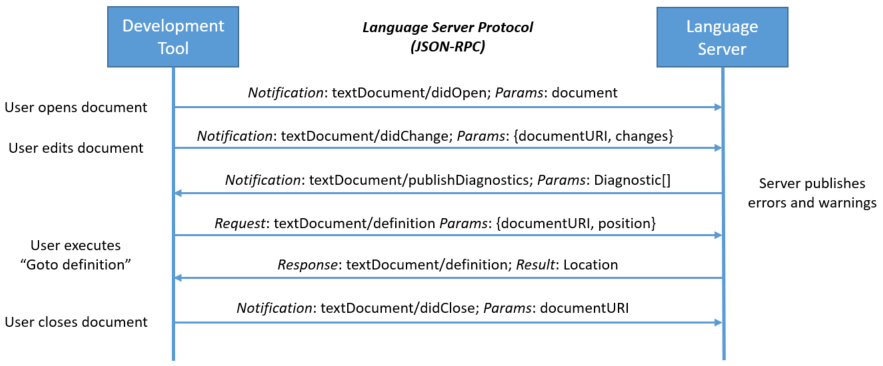
\includegraphics[width=1\textwidth]{Immagini/language-server-sequence.jpg}
	\caption{An example of communication between a tool and a Language Server through Language Server Protocol \cite{LanguageServerProtocolWebsite}}
	\label{fig:language-server-sequence}
\end{figure}

\section{The protocol}\label{sec:cap_sec_subsec}
The last version of the LSP at the time of this writing and the one that has been used in the proof-of-concept is 3.17.
The base protocol consists of a header and a content part (similar to HTTP). The header and content part are separated by a `\textbackslash r\textbackslash n'.
The header part consists of header fields which conform to the HTTP semantics. Currently the only header fields supported are Content-Length	 and Content-Type.
The content part, instead, contains the actual content of the message. This is used to send messages over JSON-RPC to describe requests, responses and notifications.

\begin{lstlisting}[caption={textDocument/didOpen notification example}, label={lst:block_struct}]
Content-Length: ...\r\n
\r\n
{
	``jsonrpc": ``2.0",
	``id": 1,
	``method": ``textDocument/didOpen",
	``params": {
		``textDocument": {
			``uri": ``file:///home/test-user/project/main.c",
			``languageId": ``c",
			``version": 1.
			``text": ``int main() { ... }"
		}
	}
}
\end{lstlisting}

\begin{lstlisting}[caption={workspace/executeCommand request example}, label={lst:block_struct}]
Content-Length: ...\r\n
\r\n
{
	``jsonrpc": ``2.0",
	``id": 1,
	``method": ``workspace/executeCommand",
	``params": {
		``command": ``trigger-analysis",
		``arguments": [``file:///home/test-user/project/main.c"]
	}
}
\end{lstlisting}

Not every Language Server can support all features defined by the protocol. LSP therefore provides \emph{capabilities}, so that both  the development tool and the Language Server can announce their supported features using capabilities at the beginning of the communication (during the ``initialize'' request). Once the capabilities of each participant in the communication are exchanged, the client and the Language Server can begin to send over requests, responses and notifications accordingly.

\section{Document Synchronization}\label{sec:cap_sec_subsec}
Each LSP client supports ``textDocument/didOpen'', ``textDocument/didChange'' and ``textDocument/didClose'' notifications. These are used by the Language Server to keep an internal synced version of the files the user is viewing. This allows the Language Server to react to changes to the file and reference specific parts of the document. For example, whenever the notification ``textDocument/didChange'' is received we can safely assume that parts of the file referenced in the notification have been changed. The LSP specification refers to three kind of document synchronization:
\begin{itemize}
  \item none, disabling all kind of document syncing;
  \item full, which means that documents are synced by always sending the full content;
  \item incremental, which means that, after sending the full content on file opening, only incremental updates to the document are sent.
\end{itemize}
In the scope of this thesis, the notification ``textDocument/didSave'' has been largely used. Below its params interface structure can be observed. 

\clearpage

\begin{lstlisting}[caption={DidSaveTextDocumentParams interface \cite{LanguageServerProtocolWebsite}}, label={lst:block_struct}]
interface DidSaveTextDocumentParams {
	/**
		* The document that was saved.
		*/
	textDocument: TextDocumentIdentifier;

	/**
		* Optional the content when saved. Depends on the includeText value
		* when the save notification was requested.
		*/
	text?: string;
}	
\end{lstlisting}

\section{Language features}\label{sec:cap_sec_subsec}
Language Features provide the actual smarts in the Language Server Protocol. Usually executed on a [text document, position] tuple, the main language feature categories are:
\begin{itemize}
	\item code comprehension features like hover or goto definition;
	\item coding features like diagnostics, code complete or code actions.
\end{itemize}
Diagnostics in particular have been the main feature used in the context of this project. In the first conceptualization of the LSP, they were something that the server could only publish to the client which were then ``owned'' by the server only, so that they were its responsibility to clear if necessary. When a file changes, it is the server's responsibility to re-compute diagnostics and push them to the client.
This approach has the advantage that for workspace-wide diagnostics the server has the freedom to compute them at a server preferred point in time. 

However, with such an approach, the server can't prioritize the computation for the file in which the user types or which are visible in the editor. Therefore, the concept of diagnostic pull requests was introduced in order to give a client more control over the documents for which diagnostics should be computed and at which point in time.
\begin{lstlisting}[caption={Diagnostic interface \cite{LanguageServerProtocolWebsite}}, label={lst:block_struct}]
export interface Diagnostic {
	/**
	 * The range at which the message applies.
	 */
	range: Range;

	/**
	 * The diagnostic's severity. Can be omitted. If omitted it is up to the
	 * client to interpret diagnostics as error, warning, info or hint.
	 */
	severity?: DiagnosticSeverity;

	/**
	 * The diagnostic's code, which might appear in the user interface.
	 */
	code?: integer | string;

	/**
	 * An optional property to describe the error code.
	 *
	 * @since 3.16.0
	 */
	codeDescription?: CodeDescription;

	/**
	 * A human-readable string describing the source of this
	 * diagnostic, e.g. `typescript' or `super lint'.
	 */
	source?: string;

	/**
	 * The diagnostic's message.
	 */
	message: string;

	/**
	 * Additional metadata about the diagnostic.
	 *
	 * @since 3.15.0
	 */
	tags?: DiagnosticTag[];

	/**
	 * An array of related diagnostic information, e.g. when symbol-names within
	 * a scope collide all definitions can be marked via this property.
	 */
	relatedInformation?: DiagnosticRelatedInformation[];

	/**
	 * A data entry field that is preserved between a
	 * `textDocument/publishDiagnostics' notification and
	 * `textDocument/codeAction' request.
	 *
	 * @since 3.16.0
	 */
	data?: unknown;
}
\end{lstlisting}


\part{The Proof of Concept}\label{part:the-proof-of-concept}
In this part of the thesis, the main results of our work are presented. 
\\\\
First, in Chapter~\ref{chapter:starting-point}, the starting point is presented: current tools and ECLAIR reports fruition are analyzed.
\\\\
Chapter~\ref{chapter:the-first-experiment} briefly describes the first experiment with the Language Server Protocol and ECLAIR, detailing the issues we faced. It laid the foundations for the prototype described in Chapter~\ref{chapter:project-architecture}.
\\\\
In Chapter~\ref{chapter:project-architecture}, the architecture of the project is presented. After a first high-level view of the interactions between the components, each of them is presented and analyzed in detail.

\chapter{Starting point}\label{chapter:starting-point}
Before moving to an in-depth analysis of what we realized, it is important to understand the starting point from which the idea of such a project was born.
ECLAIR is already widely used in many contexts in which static analysis is mandatory and enforced by standard regulations. Currently, the developers run ECLAIR on their desktop through a GUI or a CLI. 
\begin{figure}[ht]
	\centering
	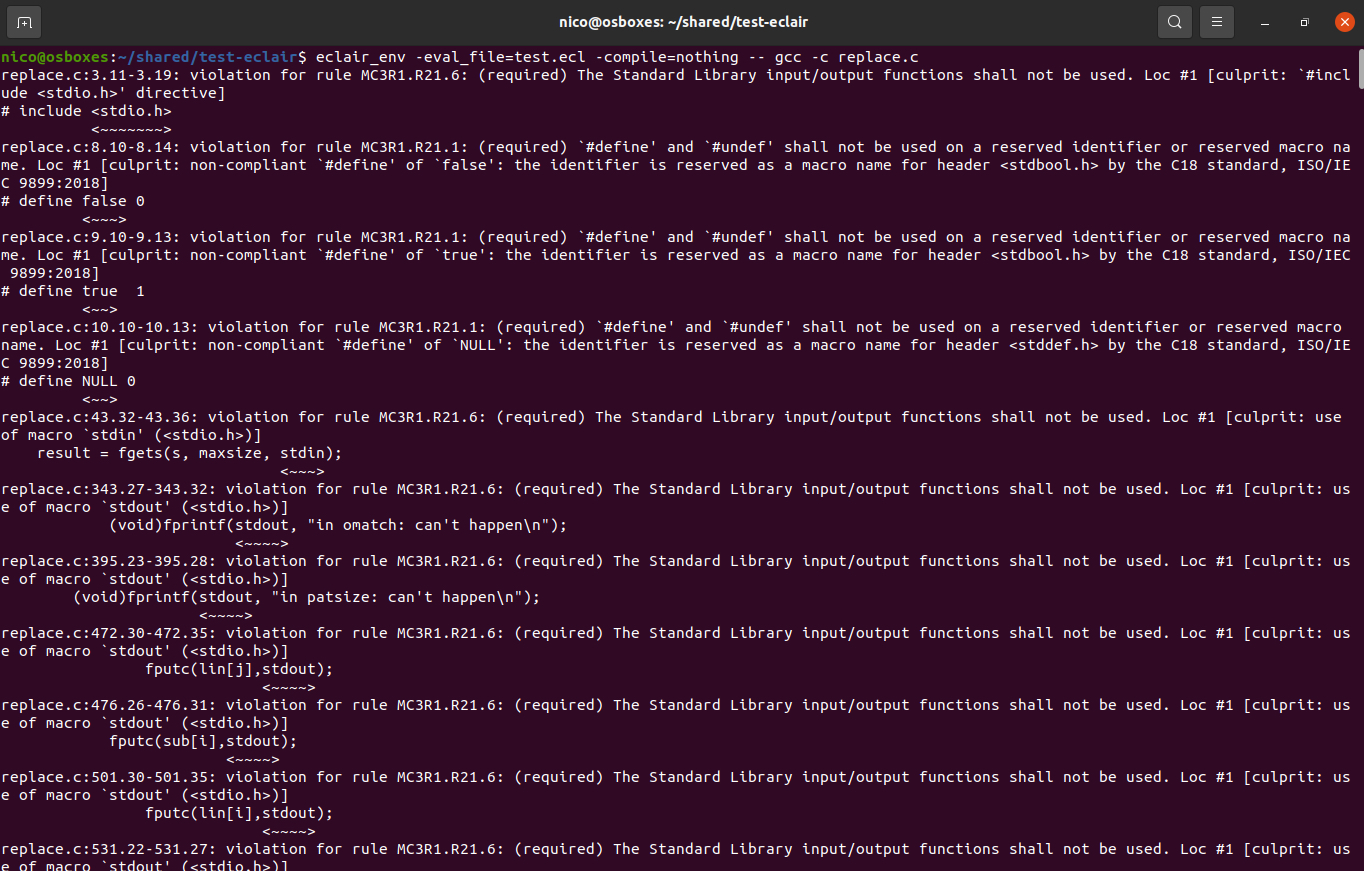
\includegraphics[width=1\textwidth]{Immagini/eclair_cli.jpg}
	\caption{ECLAIR CLI}
	\label{fig:one}
\end{figure}

In particular the first step in ECLAIR setup is configuring the toolchain, that means to indicate installed tools such as compilers and linkers: this is required since the kind of analysis that is performed is bound to the way the software is compiled. 

In addition, ECLAIR needs a \emph{.ecl} file in which rules can be activated or disabled and the report format is specified. 

\begin{lstlisting}[caption={Example \emph{.ecl} file}, label={lst:block_struct}]
-project_root=getenv(``ECLAIR_PROJECT_ROOT")

-enable=B.REPORT.TXT
-enable=MC3R1.R
-disable=`sav&&!B'
# -enable=MC3R1.R8.13

-frames={hide,`kind(object||program||project)'}

# Hides all reports that have all areas external to project root tree.
-reports+={hide,all_exp_external}
\end{lstlisting}

After the analysis, ECLAIR can produce different kinds of outputs:
\begin{itemize}
  \item summary outputs, which contain comprehensive information about the analysis, as well as counts of the issues uncovered by the analysis per service, per file, per tag and combinations;
  \item rich outputs, which contain comprehensive information about the analysis results without going into the detail of each reported program condition;
  \item detailed outputs, which contain comprehensive information about the analysis results, including all details about each reported program condition (such as a coding rule violation or a possible run-time error) and all the information required for a proper understanding of each individual issue reported by the analysis;
  \item metric outputs, which contain the values of the metrics collected for each file, function and project.
\end{itemize}

These outputs can be returned in different formats:
\begin{itemize}
  \item summary and rich outputs in printable format (\emph{.odt} or \emph{.doc}), HTML format or pure text;
  \item rich interactive outputs in spreadsheet format, which contain the set of ECLAIR findings in a form that is suitable for the communication to third parties that are only interested in the residual violations and whether they have been justified and how;
  \item detailed outputs in interactive spreadsheet format, pure text format or printable format.
\end{itemize}

\begin{figure}[ht]
	\centering
	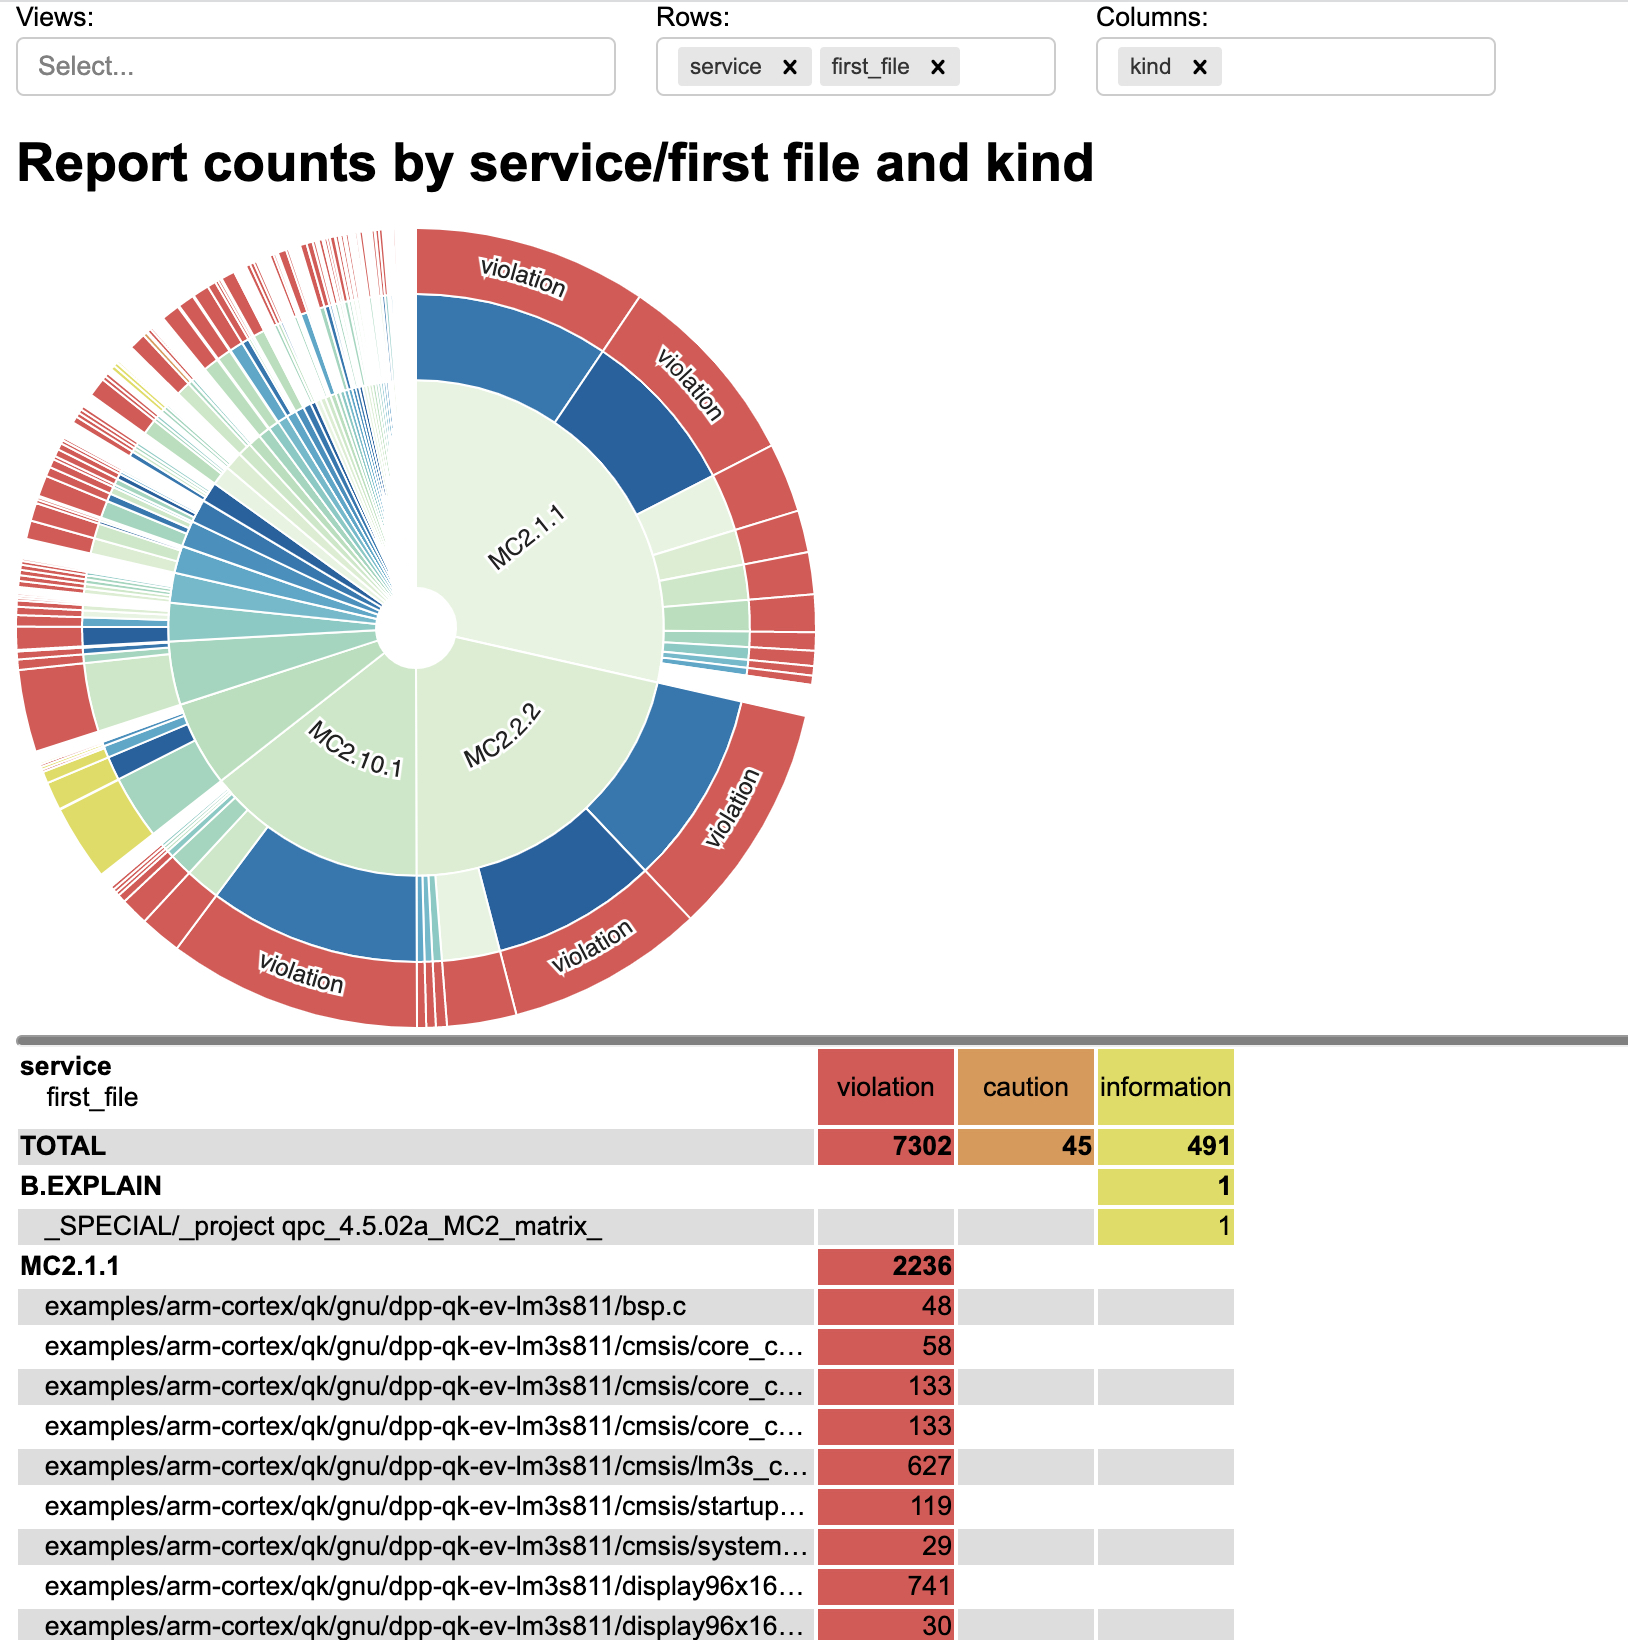
\includegraphics[width=1\textwidth]{Immagini/eclair_rich_output_html.jpg}
	\caption{Example of ECLAIR rich output in HTML format}
	\label{fig:one}
\end{figure}

Since static analysis integration in continuous integration pipelines is a must-have in modern development, the eclairit.com web site was created. This demonstrates the use of ECLAIR integrated into Jenkins\footnote{https://www.jenkins.io} and GitLab. An integration server performs the analysis and provides the reports directly in the browser, without having to install ECLAIR on each PC. This was the first change of paradigm from the traditional analysis performed directly on developers' machines.
This tool gave us the inspiration to integrate ECLAIR in the development workflow in a new way: we wanted to perform the analysis while the users were writing the code.

\begin{figure}[ht]
	\centering
	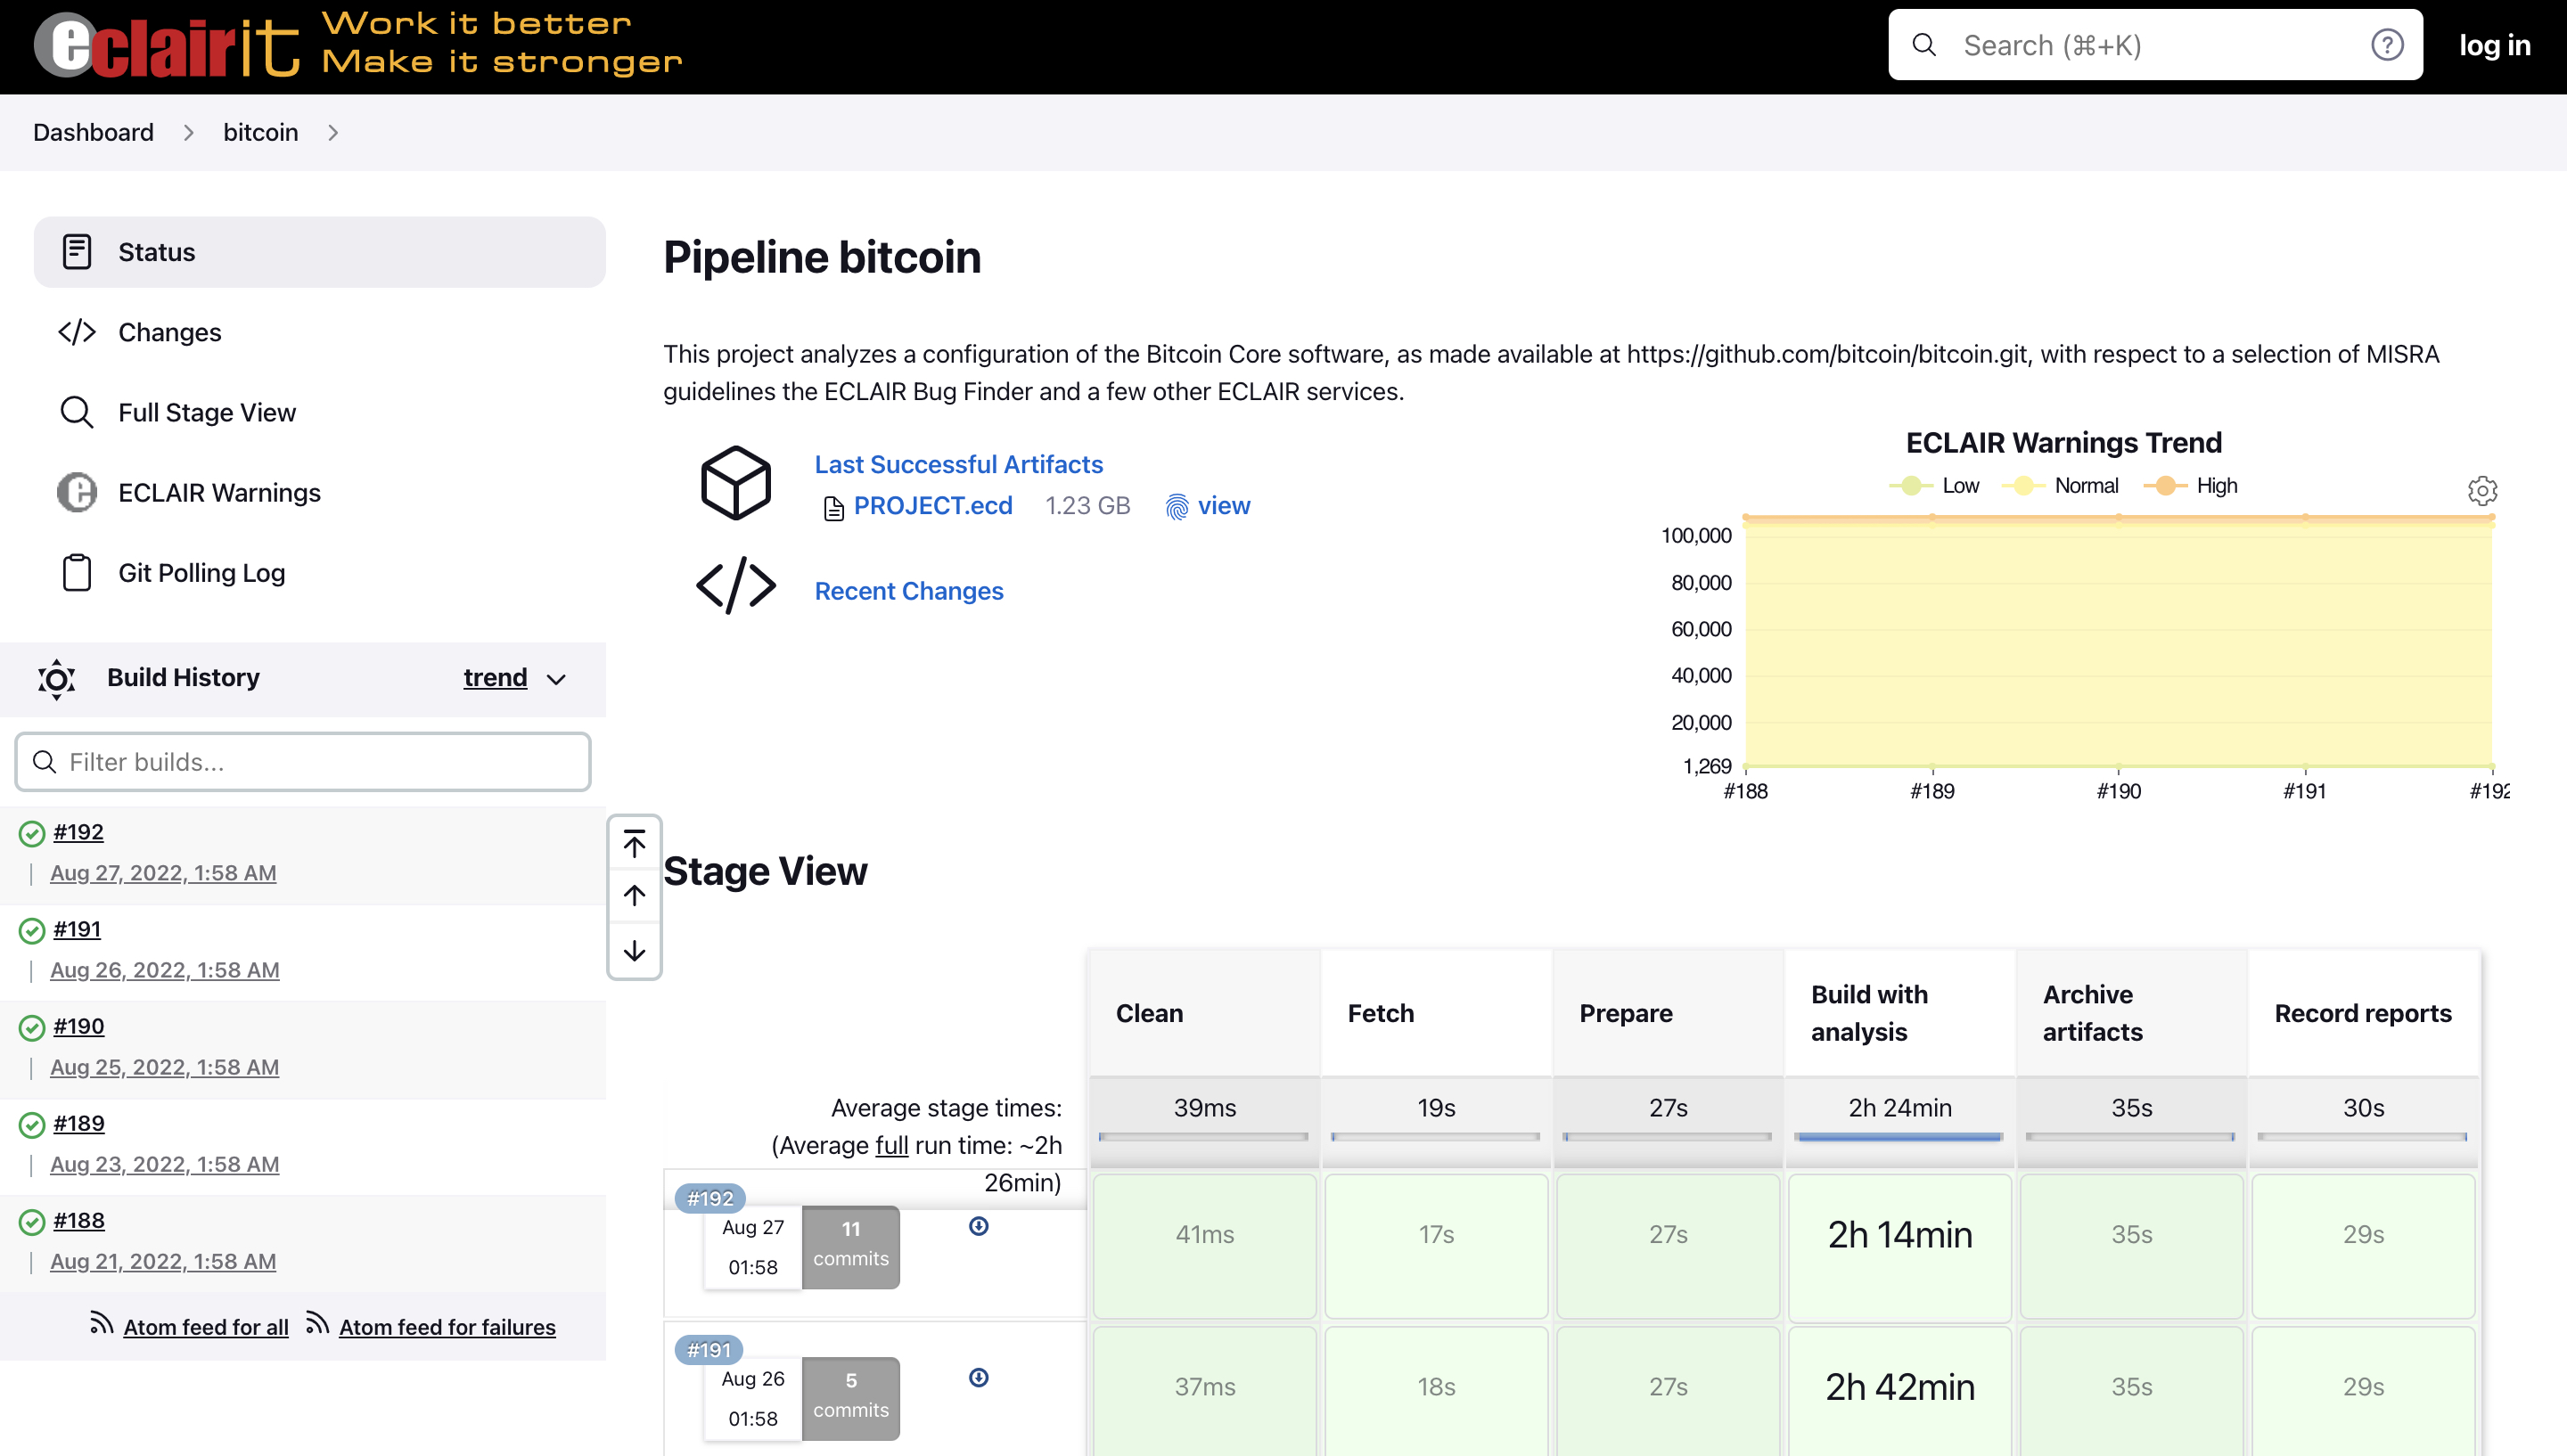
\includegraphics[width=1\textwidth]{Immagini/eclairit.jpg}
	\caption{eclairit.com}
	\label{fig:one}
\end{figure}
\chapter{The first experiment}\label{chapter:the-first-experiment}
When we first thought about using the LSP in this project we decided to try it first hand with a simple implementation of the ECLAIR analysis in the IDE. The first iteration consisted of a Language Server which simply listened to file changes which would in turn trigger a new ECLAIR analysis each time using the CLI. Then the analysis output would be parsed, converted to LSP Diagnostics and sent over to the client. 

\begin{figure}[ht]
	\centering
	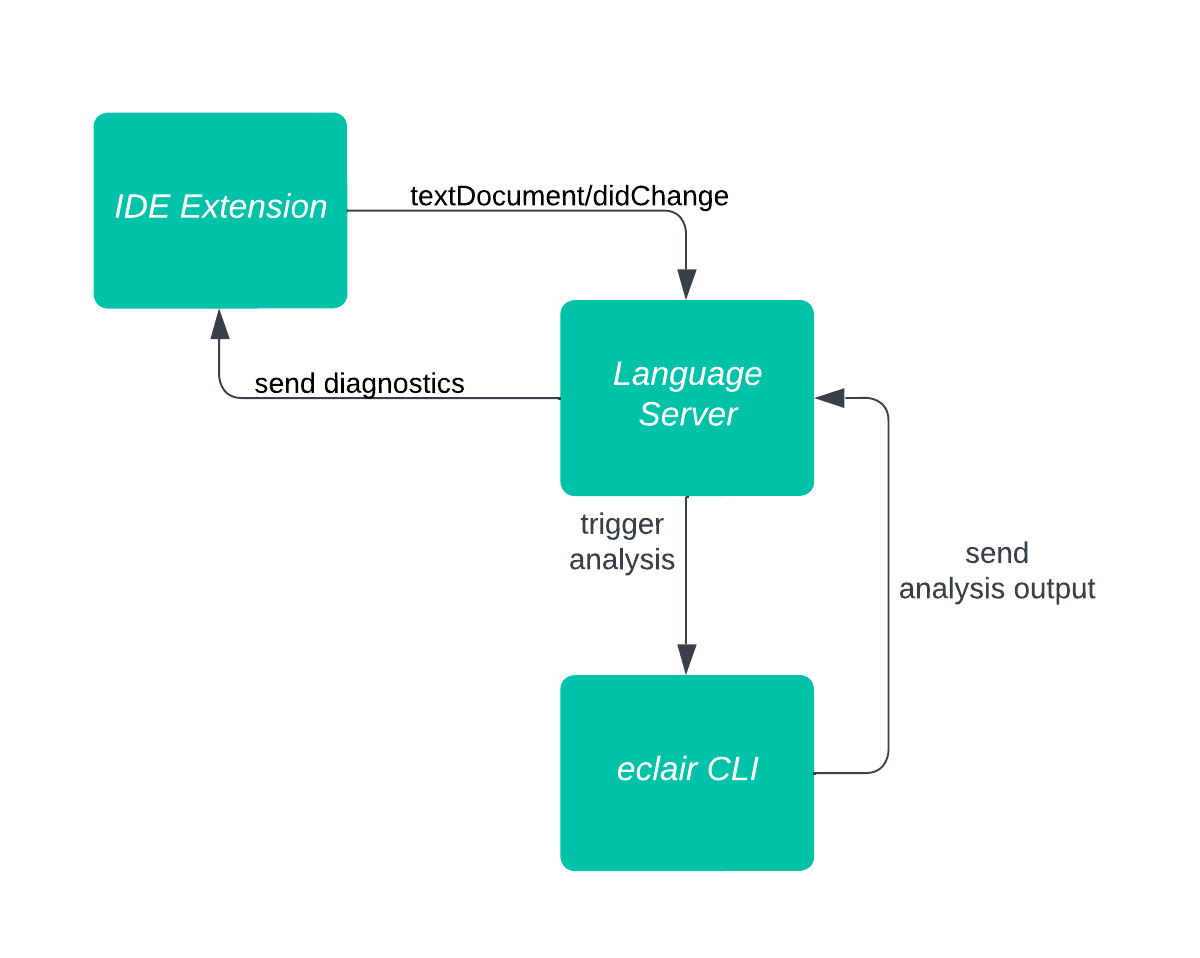
\includegraphics[width=0.9\textwidth]{Immagini/the_first_experiment_flow.jpg}
	\caption{First experiment with the Language Server Protocol}
	\label{fig:one}
\end{figure}

\clearpage

In order to fully understand the benefits the LSP could give us, we realized two extensions, for VSCode and Sublime Text. In both cases we could observe that, with just a few lines, we were able to see the violations marked in the file.

\begin{lstlisting}[caption={First Sublime Text working configuration}, label={lst:block_struct}]
{
  ``clients": {
    ``elcair": {
      ``command": [
        ``eclair-server",
        ``--stdio"
      ],
      ``enabled": true,
      ``languages": [
        {
          ``languageId": ``c"
        }
      ]
    }
  },
  ``log_debug": true
}
\end{lstlisting}

\begin{lstlisting}[caption={First VSCode working extension}, label={lst:block_struct}]
const { LanguageClient } = require(``vscode-languageclient")

module.exports = {
  activate(context) {
    const executable = {
      command: ``eclair-server",
      args: [``--stdio"]
    }

    const serverOptions = {
      run: executable,
      debug: executable
    }

    const clientOptions = {
      documentSelector: [{
        scheme: ``file",
        language: ``c"
      }]
    }

    const client = new LanguageClient(
      ``eclair-extension-id",
      ``Eclair",
      serverOptions,
      clientOptions
    )

    context.subscriptions.push(client.start())
  }
}
\end{lstlisting}
\chapter{Project architecture}\label{chapter:project-architecture}
This chapter presents the prototype we realized and the reasons behind some choices. The main components analyzed here are:
\begin{itemize}
  \item \emph{eclair};
  \item \emph{eclair\textunderscore	report};
  \item a Language Server;
  \item the VSCode extension.
\end{itemize}
The following diagram aims at giving a high-level overview of the components and their interactions: each process will be analyzed in-depth in the following sections. 

However, it is already possible to understand the neat division between the IDE extension, the Language Server and the analysis services. Through the LSP, the IDE communicates to the Language Server, which in turn invokes the \emph{eclair} CLI to perform the analysis or asks \emph{eclair\textunderscore	report} for interesting violations given the current viewport.

\begin{figure}[ht]
	\centering
	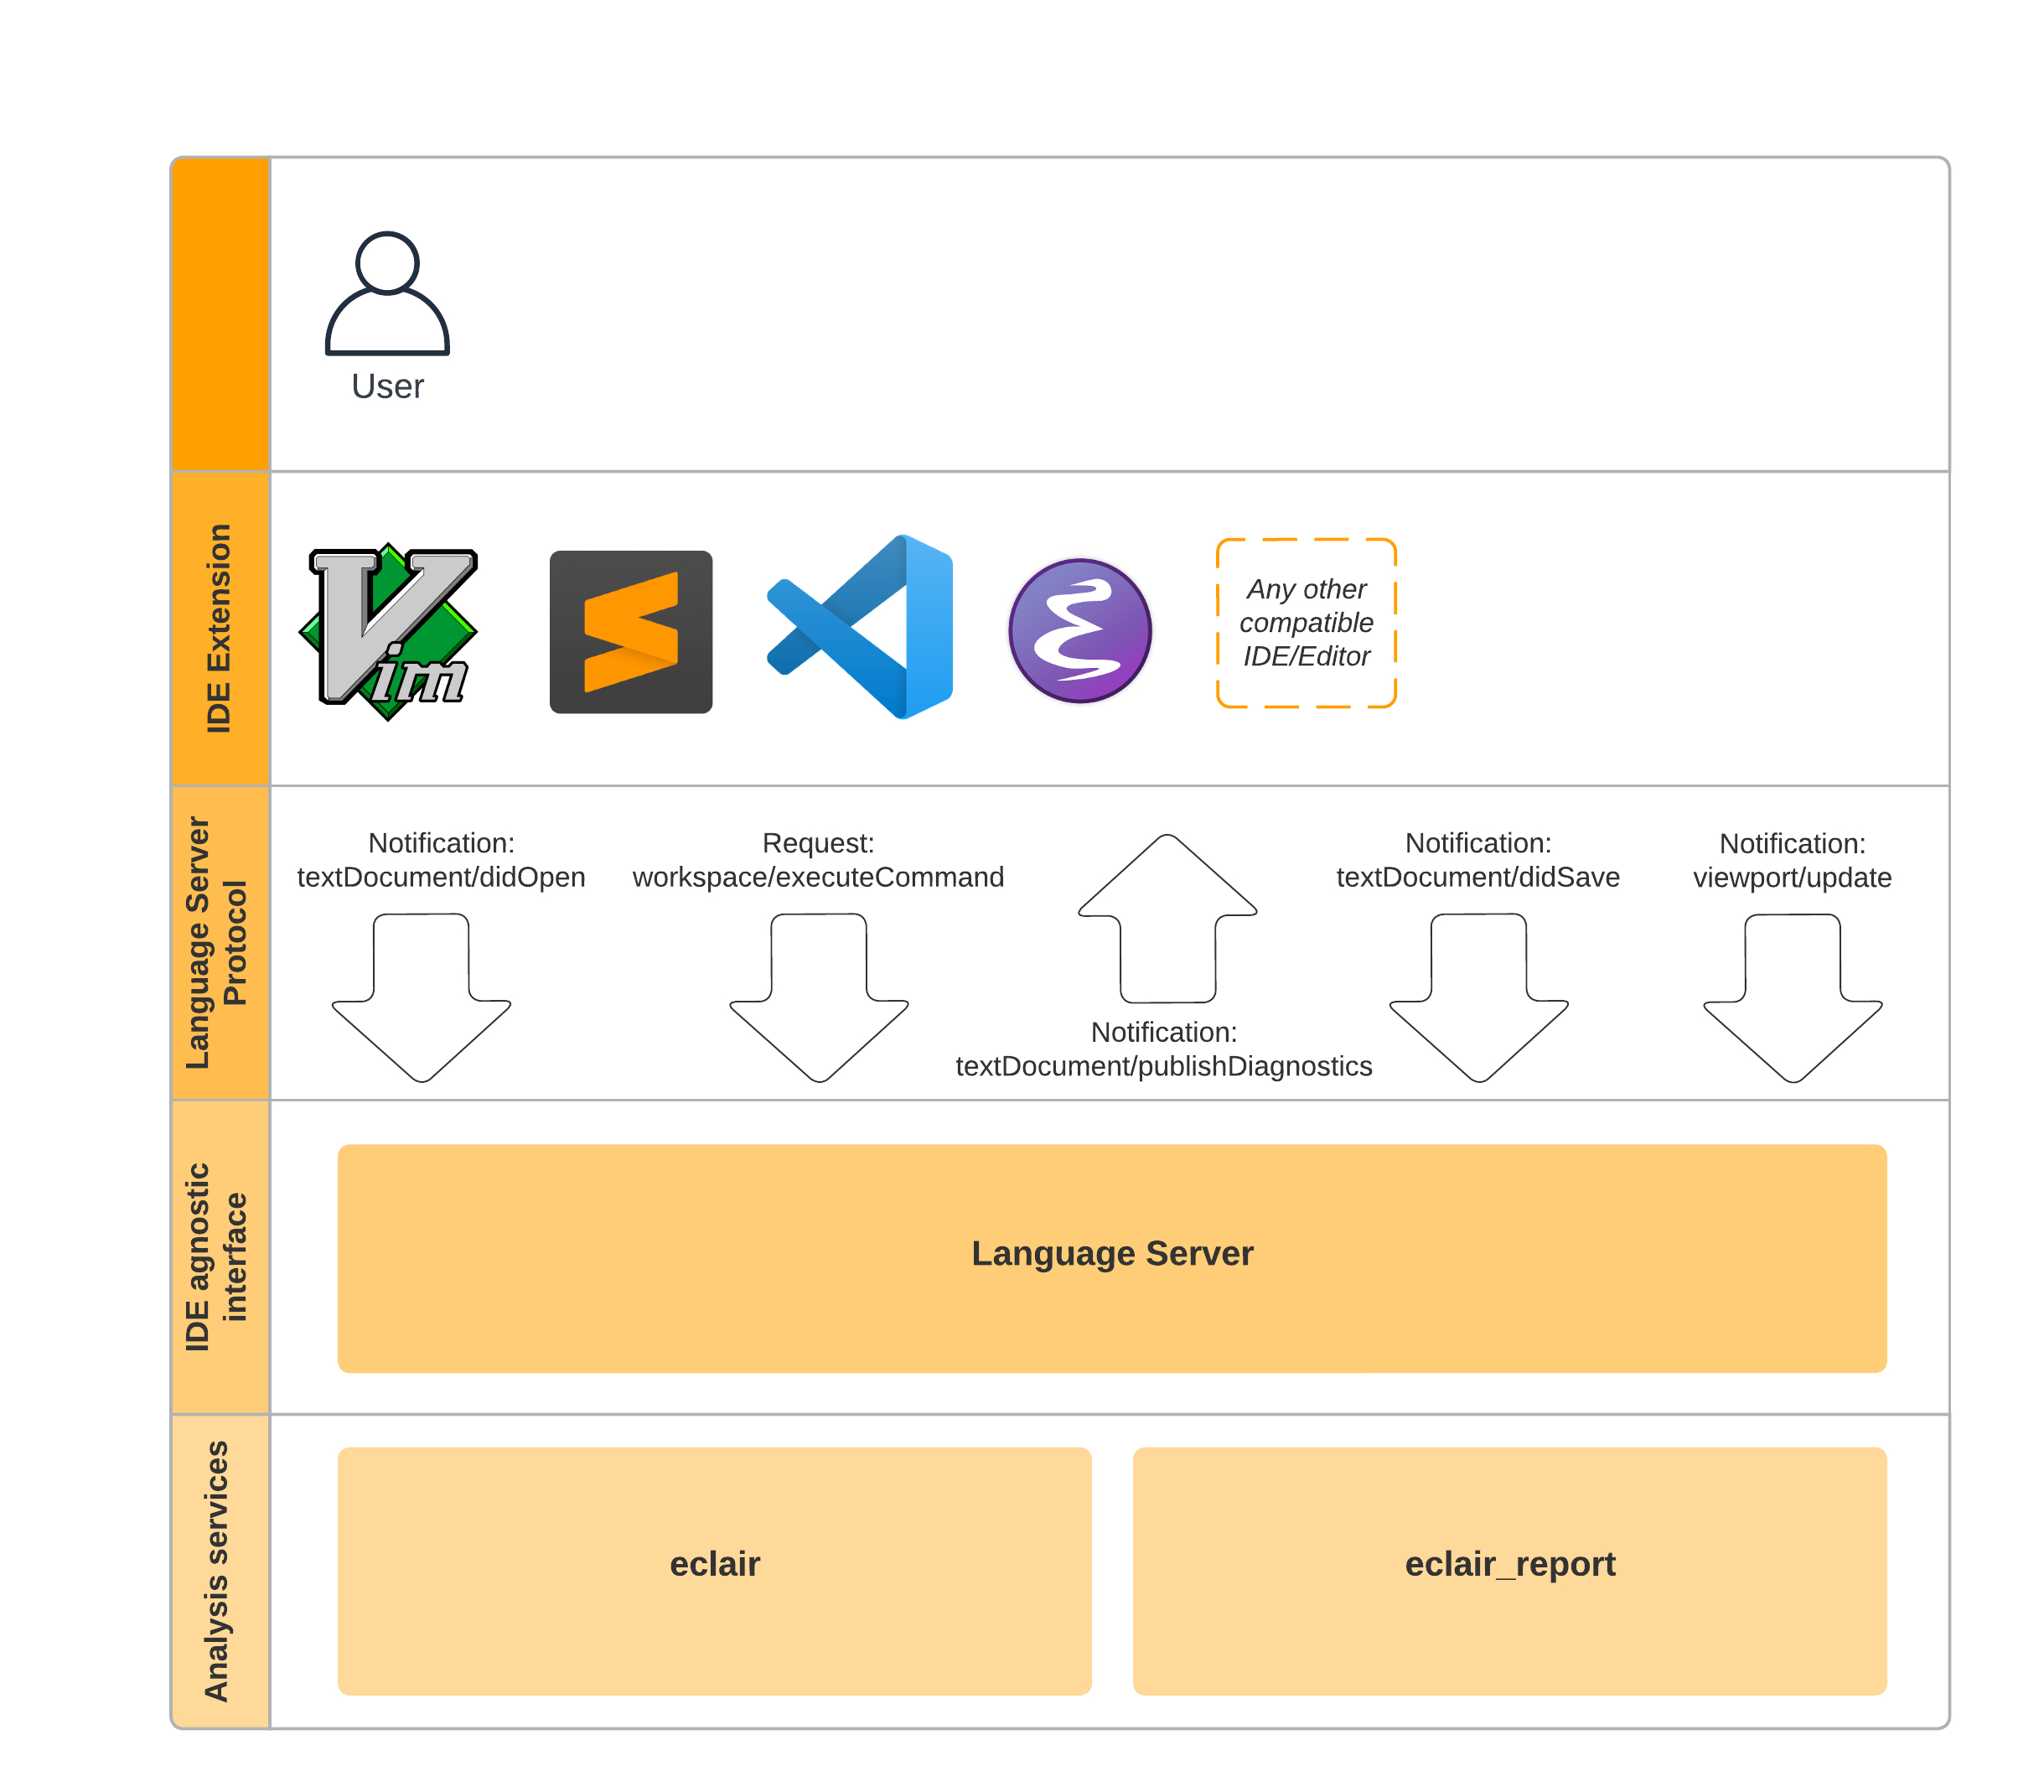
\includegraphics[width=1\textwidth]{Immagini/project_architecture.jpg}
	\caption{Project architecture}
	\label{fig:one}
\end{figure}

The Language Server uses the output received from \emph{eclair\textunderscore	report} to communicate to various IDE extensions, through the LSP, what must be shown to the end user. 

The separation of concerns and the decoupling of the components is at the foundation of this architecture: \emph{eclair\textunderscore	report} is expected to care only about serving the violations to the Language Server, while the \emph{eclair} CLI performs the analysis in an agnostic way regarding how the violations will be served. The only interface the IDE extension has to deal with is the Language Server, which is always the same, independently from the IDE, and hides the complexity of implementing the calls to the analysis services. This way, building new extensions for other IDEs is painless and, with just a few lines of code, it is possible to communicate with the Language Server from the earlier stages of the development. On top of these foundations, extension developers can concentrate on providing the best experience to the end users without worrying about linking the analysis tools to the dishomogeneous IDEs' primitives and APIs.

\section{\emph{eclair}}\label{sec:cap_sec_subsec}
The \emph{eclair} CLI is used to invoke the static analyzer. In order for ECLAIR to work, there must exist an \emph{.ecl} file that specifies:
\begin{itemize}
  \item project-specific configurations;
  \item MISRA rules that should be checked for compliance;
  \item report output format.
\end{itemize}

So the first thing before proceeding with the analysis, is to check for an existing \emph{.ecl} file in the project directory.
\\\\
There are three occasions in which the Language Server invokes the \emph{eclair} CLI:
\begin{itemize}
  \item a new file is opened for the first time;
  \item changes to a file are saved (the user can opt out of this feature);
  \item an analysis is manually triggered.
\end{itemize}

The first two cases are handled automatically whenever the Language Server receives the corresponding notifications, respectively \emph{``textDocument/didOpen''} and \emph{``textDocument/didSave''}. The third case, instead, relies on a \emph{``workspace/executeCommand''} request that is sent from the IDE extension to the Language Server.
\\\\
After performing an analysis, the \emph{eclair} CLI sends its findings to \emph{eclair\textunderscore	report} which in turn saves them into a project internal database, in \emph{.ecd} format. This database will then be used by \emph{eclair\textunderscore	report} to provide the violations.

\begin{figure}[ht]
	\centering
	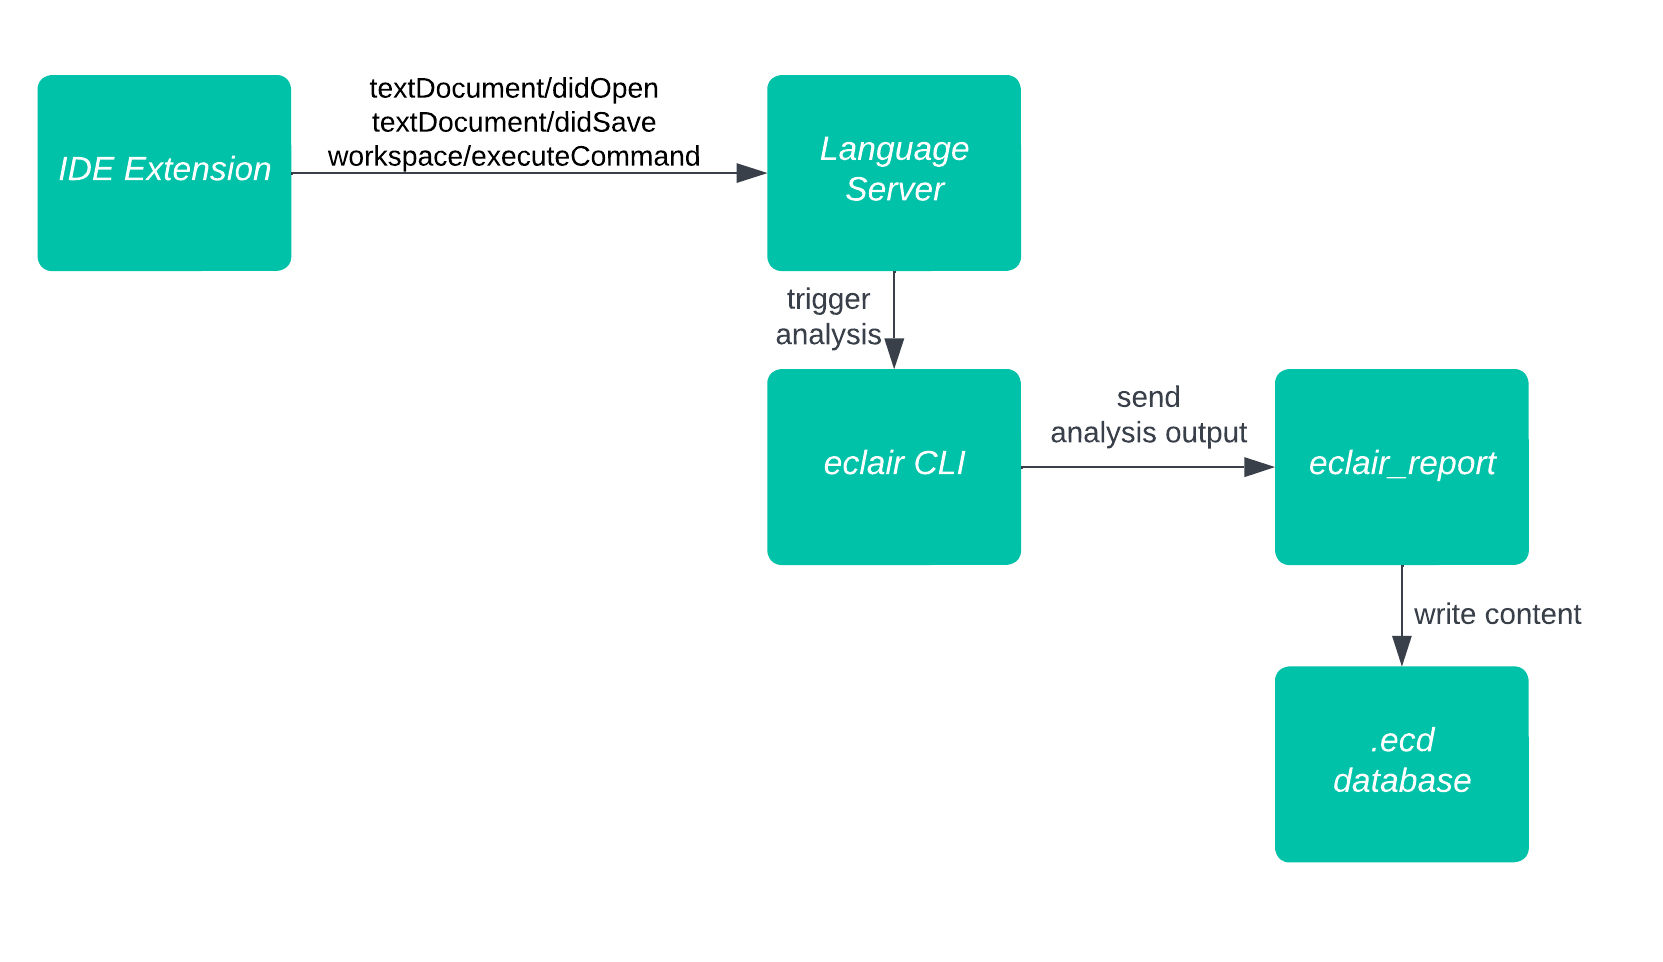
\includegraphics[width=1\textwidth]{Immagini/eclair_analyzer_flow.jpg}
	\caption{Interaction with the \emph{eclair} CLI}
	\label{fig:one}
\end{figure}

\section{\emph{eclair\textunderscore	report}}\label{sec:cap_sec_subsec}
\emph{eclair\textunderscore	report} is already part of the ECLAIR ecosystem: its job is to export ECLAIR analysis findings to different formats (more details about the currently available formats can be found in Chapter~\ref{chapter:starting-point}). 
In the first experiment, described in Chapter~\ref{chapter:the-first-experiment}, the analysis was performed from the beginning whenever the user changed something in the file and violations were returned all at once: unfortunately we noticed that this approach resulted in a slow feedback to the user and sometimes useless analyses were performed. 
\\\\
We decided to use a combination of \emph{eclair} and \emph{eclair\textunderscore	report} to perform the analysis only when necessary and serve its output incrementally. 
The first thing \emph{eclair\textunderscore	report} has to do in our architecture is to save the analysis findings in the project level \emph{.ecd} database. 

Once we had established this, we could build on top of this database features like incrementality and various optimization for the following analyses.
After some reasoning, we decided to proceed with the first, and postpone for now the latter. 

Returning all the violations all at once to the IDE wasn't optimal in particular for huge files: we had to find a new way to navigate them.
We designed a new feature of \emph{eclair\textunderscore	report} that would allow us to interrogate the service and ask incrementally the violations recorded: when interrogated, the tool would be able to receive a top line index and bottom line index and return only the violations in the given range.
Hence, keeping an updated internal state in the Language Server with the current user viewport, we could achieve the incrementality we aimed at. 

\begin{figure}[ht]
	\centering
	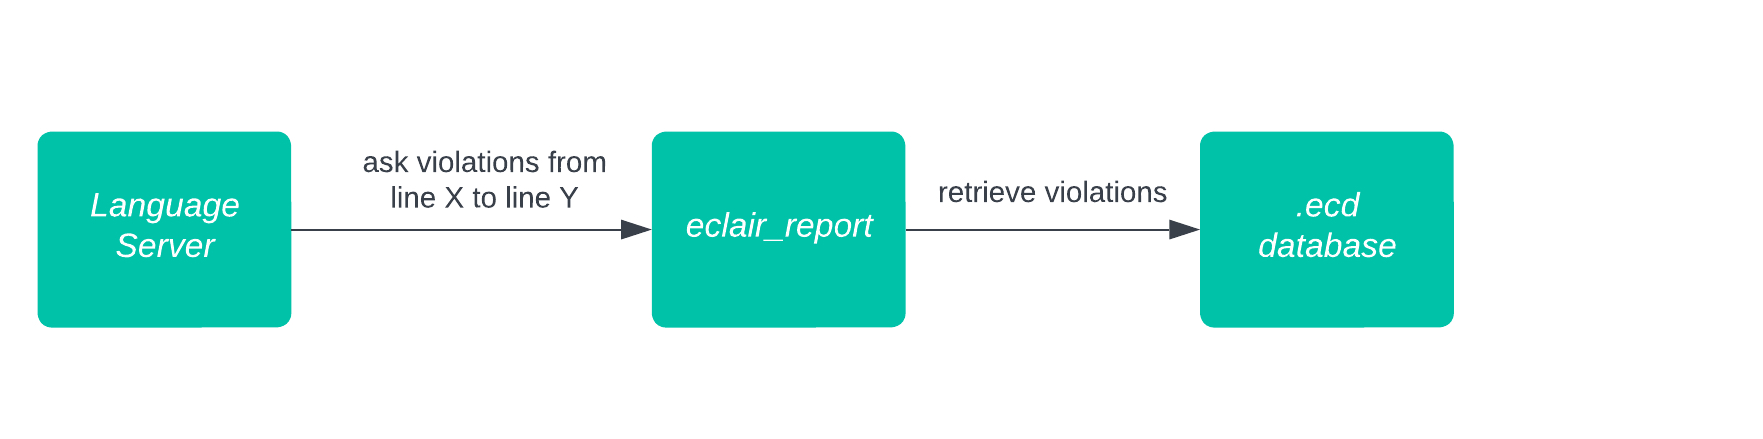
\includegraphics[width=1\textwidth]{Immagini/eclair_report_flow.jpg}
	\caption{Interaction with \emph{eclair\textunderscore	report}}
	\label{fig:one}
\end{figure}

\section{Language Server}\label{sec:language_server_component}
The Language Server is a software written in Typescript, a superset of JavaScript that adds optional static typing to the language, that runs on NodeJS and behaves like a bridge between the ECLAIR ecosystem and the IDE.

In particular, it relies on an implementation of the LSP provided as an NPM library from Microsoft, \lstinline{vscode-languageserver}\footnote{https://www.npmjs.com/package/vscode-languageserver}, and makes the calls to \emph{eclair} and \emph{eclair\textunderscore	report}. 

The Language Server saves an internal representation of the document the user is looking at, incrementally updates it during the editing, and uses it to mark violations.
Every time the user saves the file, opens a new one or manually triggers an analysis a message is sent over to the Language Server, which in turn will trigger an execution by the \emph{eclair} CLI. To avoid useless invocations, the file savings are batched for a defined period of time before making the call asking to perform the analysis.
\begin{lstlisting}[caption={Server side code for viewport synchronization}, label={lst:block_struct}]
type Viewport = {
	filename: string
	topLineIndex: number
	bottomLineIndex: number
}

let viewport: Viewport
const BUFFER = 20

connection.onNotification((method, params) => {
	if (method === ``viewport/update") {
		viewport = params as Viewport

		const uri = ``file://${viewport.filename}"

		connection.sendDiagnostics({
			uri,
			diagnostics: eclairReports.getViolations(workspaceFolder, uri, viewport.topLineIndex - BUFFER, viewport.bottomLineIndex + BUFFER)
		})
	}
})
\end{lstlisting}

\begin{lstlisting}[caption={VSCode extension side code for viewport synchronization}, label={lst:block_struct}]
let lastRecorded = {
	filename: null,
	topLineIndex: null,
	bottomLineIndex: null
}

let timeout: NodeJS.Timeout
Window.onDidChangeTextEditorVisibleRanges(() => {
	if (timeout) {
		clearTimeout(timeout)
	}
	timeout = setTimeout(() => {
		const textEditor = Window.activeTextEditor
		if (textEditor) {
			const visibleRange = textEditor.visibleRanges[0]
			const filename = textEditor.document.fileName
			const topLineIndex = visibleRange.start.line
			const bottomLineIndex = visibleRange.end.line
			if (
				lastRecorded.filename !== filename ||
				lastRecorded.topLineIndex !== topLineIndex ||
				lastRecorded.bottomLineIndex !== bottomLineIndex
			) {
				lastRecorded.filename = filename
				lastRecorded.topLineIndex = topLineIndex
				lastRecorded.bottomLineIndex = bottomLineIndex
				client.sendNotification(``viewport/update", lastRecorded)
			}
		}
	}, 500)
})
\end{lstlisting}
One of the sophistications we had to adopt is the incrementality in the diagnostics: we could not send the violations all at once. However, in order to visualize only the necessary ones, the Language Server must know the file the user is currently looking at and the lines currently in the viewport. 

Unfortunately this feature is not natively offered by the LSP. Thus, inspired from the Text Document Synchronization, we opted for the following approach: whenever the user changes the current active file or viewport, the client retrieves these informations using the IDE's API and uses an LSP notification to send these details to the server, which in turn keeps an internal state. Hence, the Language Server is able to interrogate \emph{eclair\textunderscore	report} and receive only the violations for the file and the lines the user actually needs.

\begin{figure}[ht]
	\centering
	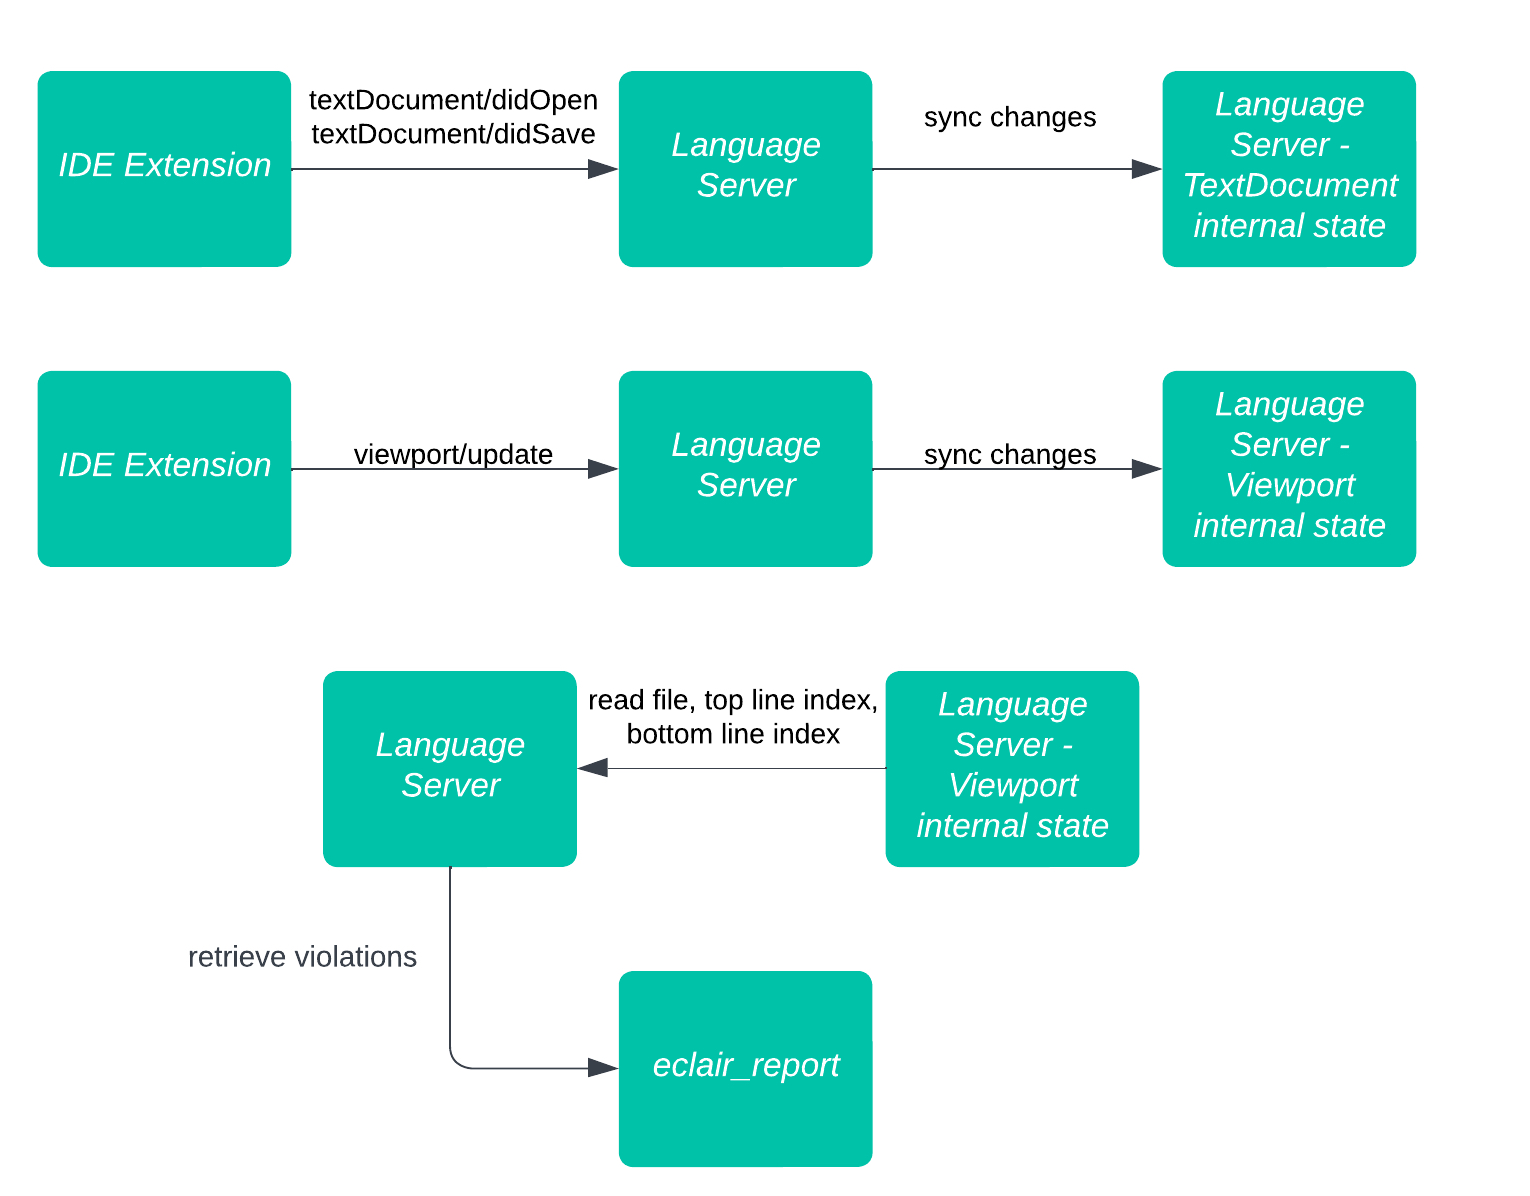
\includegraphics[width=1\textwidth]{Immagini/language_server_flow.jpg}
	\caption{Interactions with the Language Server}
	\label{fig:one}
\end{figure}

\section{VSCode extension}\label{sec:cap_sec_subsec}
The VSCode extension, which in this case exemplifies all the possible IDE plugins/extensions that can be realized on top of this system, has nearly no logic implemented. 
Its main task is the creation of the connection with the Language Server.
\\
In addition to that, some other features, not completely agnostic to the IDE, have been implemented: aside from the viewport synchronization logic, which must retrieve the current viewport using IDE's primitives, already discussed in Section~\ref{sec:language_server_component}, 
we also had to implement a way to manually trigger the analysis and give the user the possibility to opt out from the ``analysis on save'' feature.
Regarding the manually triggered analysis, the Listing~\ref{lst:trigger_analysis_command_code} should give more insights about how we linked the VSCode ``Commands.registerCommand'' API to the ``workspace/executeCommand'' request.
\begin{lstlisting}[caption={VSCode extension triggerAnalysis command}, label={lst:trigger_analysis_command_code}]
Commands.registerCommand(``eclair.triggerAnalysis", () => {
	const uri = Window.activeTextEditor.document.uri
	client.sendRequest(``workspace/executeCommand", {
		command: ``trigger-analysis",
		arguments: [uri.toString()]
	} as ExecuteCommandParams)
})
\end{lstlisting}

On the other hand, the automatic ``analysis on save'' was something we had to think through: a lot of IDEs users have autosaving configurations enabled, so we had to at least make possible to opt out of this feature, given how expensive the analysis is.
We exposed a boolean configuration, \emph{eclair.performAnalysisOnSave}, to switch off the ``analysis on save'' feature and, to fully comply with the LSP approach, we decided that the IDE extension should send over this information with the capabilities in the initialization phase.
In particular, as can be seen on line 14 of Listing~\ref{lst:extension_initialization}, all the content of \emph{Workspace.getConfiguration(``eclair'')} is sent over: if the server is able to use the forwarded settings it will, otherwise they will simply be ignored.

\begin{lstlisting}[caption={VSCode extension initialization}, label={lst:extension_initialization}]
const debugOptions = { execArgv: [``--nolazy", ``--inspect=6011"] }
const serverOptions = {
	run: { module, transport: TransportKind.ipc },
	debug: { module, transport: TransportKind.ipc, options: debugOptions }
}
const clientOptions: LanguageClientOptions = {
	documentSelector: [
		{ scheme: ``file", language: ``c", pattern: ``${folder.uri.fsPath}/**/*" }
	],
	diagnosticCollectionName: ``eclair-language-server",
	workspaceFolder: folder,
	outputChannel: outputChannel,
	progressOnInitialization: true,
	initializationOptions: Workspace.getConfiguration(``eclair")
}
const client = new LanguageClient(``eclair-vscode-client", ``ECLAIR", serverOptions, clientOptions)
client.start()
\end{lstlisting}

Extensibility is at the core of the VSCode plugin and, thanks to the LSP notification based communication, it's simple and intuitive to implement new features, even at different time, on the server and on the client.
In around 200 lines of code, our extension was fully functional and ready to be used as an inspiration to develop other extensions that use the same Language Server.
\begin{figure}[ht]
	\centering
	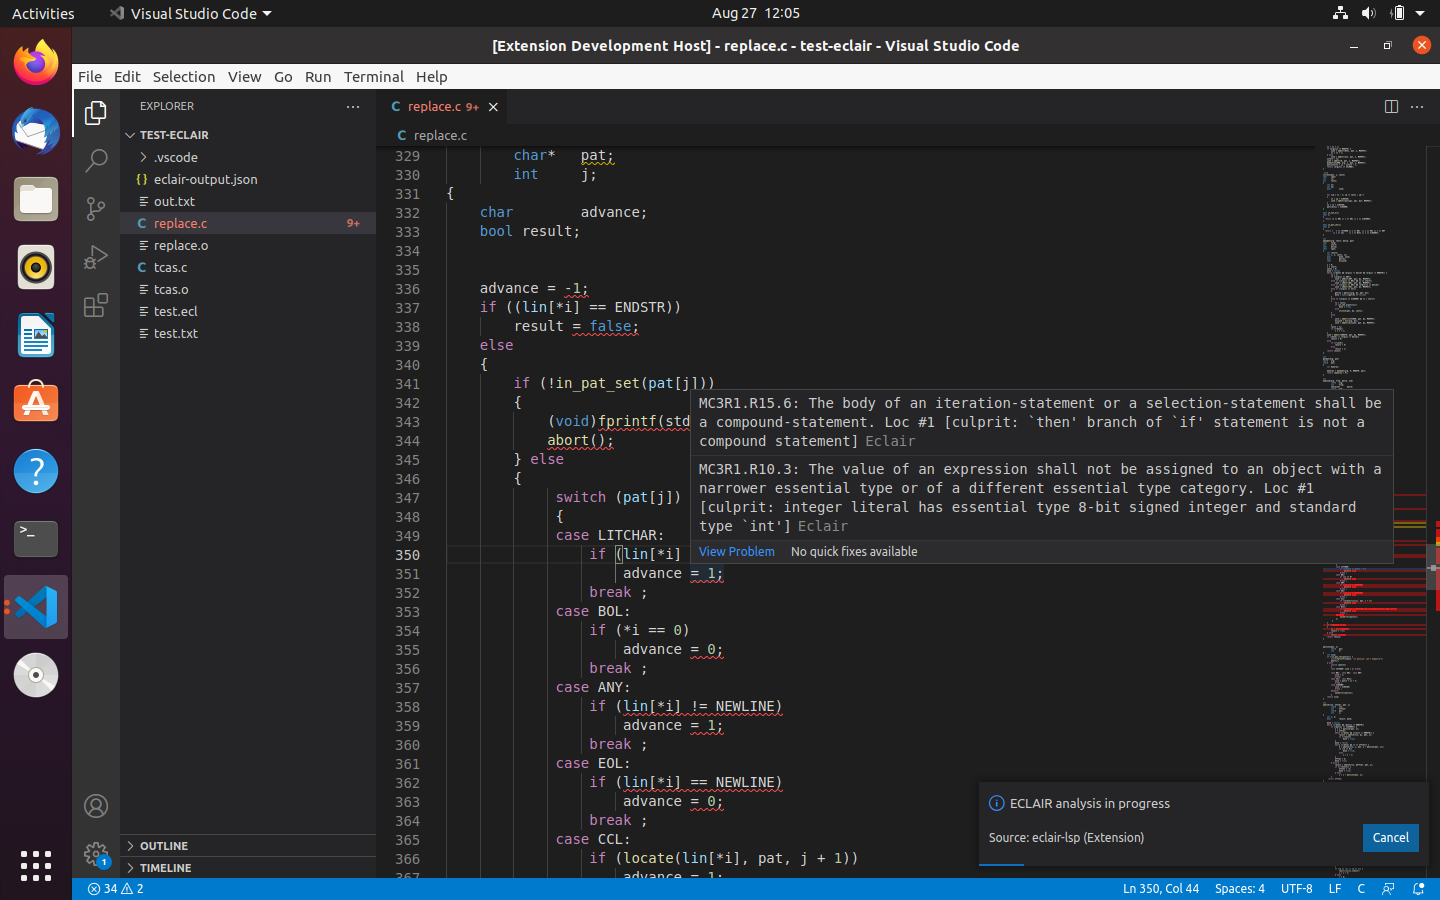
\includegraphics[width=1\textwidth]{Immagini/vscode_extension_screenshot.jpg}
	\caption{A screenshot of the VSCode extension in action}
	\label{fig:one}
\end{figure}

\part{Conclusion}
Finally, in Chapter~\ref{chapter:discussion-and-future-work} some conclusions are drawn. 
After an overview of the challenges we faced, some reasonings about future work are presented.

\chapter{Discussion and future work}\label{chapter:discussion-and-future-work}
The work we did to implement this proof-of-concept gave us a taste of the benefit a tool of this kind can be to developers: after the first analysis was performed, we could navigate smoothly through the code and receive almost instant feedback about the violations that were detected. 
The aim of this project was to determine whether this could be a feasible way to use ECLAIR analysis output and to lay the foundations of what can be a game changing tool for developers who develop safety-critical software.
\\\\
During the realization, we faced issues common to this kind of projects and found appropriate solutions: first the need for a common interface between the editors was solved using the LSP, then we relied on \emph{eclair\textunderscore	report} to answer the need for incrementality in the showing of the violations, then we achieved parallelism spawning multiple ECLAIR analysis from the Language Server when necessary and so on.
\\\\
We also had time to think about future improvements, that can make this piece of software production-ready and experiments to improve it: for example the pull diagnostics mechanism should be tested, and see if it actually could replace the current one, which pushes diagnostics from the server to the client. 

This approach would allow the client to ask for violations only when it decides they are needed and not receive them passively from the server. 

Another improvements on the side of the ECLAIR analyzer would be to reuse the previous analyses and re-analyze only what actually changed, without having to analyze the entire file. 
While this is feasible for some kinds of violations, it can be challenging for others.

At last, thanks to the decoupling granted by the Language Server Protocol, we can imagine scenarios in which the analysis is not even performed on the developer machine, but instead on a dedicated one that sends the results of the analysis through the protocol. 
At the moment of this writing the transport channel can either be stdio, sockets, named pipes, or node ipc if both the client and server are written for Node.js. 
\\\\
The leitmotif of this thesis has been the simplicity: from the very beginning we had a clear view of the components, how we wanted them to interact and the precise level of isolation each level should have from the others that resulted in a simple and elegant implementation.

One of the reasons behind this project was to assess whether the Language Server Protocol, an ever-growing standard, could actually make it possible to integrate an existing analysis tool into IDEs easily.
We think that, after developing the reusable Language Server, the only 200 lines of code that were necessary to integrate it into VSCode have been our witnesses.
\\\\
This thesis describes the underlying ideas, the challenges and the solutions explored during the implementation of this prototype. We hope that the reader had the opportunity to learn new lessons, understand the potentiality of the new technologies we used and to better understand the evolutions of the static analysis ecosystem and its tooling.


%
%%%% La bibliografia
\bibliographystyle{plain} %{apalike} -- Scegliere lo stile preferito
\nocite{*}
\bibliography{./Bibliografia}
%
\chapter*{Ringraziamenti}

\emph{Vorrei dedicare questo spazio alle persone che mi hanno supportato nella redazione di questo lavoro di tesi.\\}

\emph{Ringrazio il mio relatore Roberto Bagnara che mi ha seguito, con la sua infinita disponibilità, pronto a fornirmi strumenti, migliorie e suggerimenti utili ai fini della stesura dell'elaborato.\\}

\emph{Non posso non menzionare i miei genitori e mio fratello che da sempre mi sostengono nella realizzazione dei miei progetti.\\}

\emph{Un ringraziamento particolare va a Giovanni Bruno, Valerio Versace e Daniele Donelli, che prima come mentori e poi come soci in Soluzioni Futura, sono stati in grado di trasmettermi la loro passione per l'informatica  e con i quali affronto sfide tecnologiche sempre nuove.\\}

\emph{Ringrazio Claudia Chiarenza, per essere stata sempre presente, per il suo supporto e incoraggiamento ad ogni passo di questo percorso.\\}

\emph{Ringrazio inoltre Abramo Bagnara e Simone Ballarin di BUGSENG per i momenti di confronto, i contributi nel design del progetto e per la realizzazione dell'ecosistema ECLAIR.\\}

\emph{Grazie a tutti i miei colleghi di corso, per avermi sempre incoraggiato fin dall'inizio del percorso universitario e per tutti i momenti di spensieratezza.\\}

\emph{Infine, vorrei dedicare questo traguardo anche a me stesso, che possa essere l'inizio di una lunga e brillante carriera professionale.}
%
\end{document}